\documentclass[11pt,]{article}
\usepackage[left=1in,top=1in,right=1in,bottom=1in]{geometry}
\newcommand*{\authorfont}{\fontfamily{phv}\selectfont}
\usepackage[]{mathpazo}


  \usepackage[T1]{fontenc}
  \usepackage[utf8]{inputenc}



\usepackage{abstract}
\renewcommand{\abstractname}{}    % clear the title
\renewcommand{\absnamepos}{empty} % originally center

\renewenvironment{abstract}
 {{%
    \setlength{\leftmargin}{0mm}
    \setlength{\rightmargin}{\leftmargin}%
  }%
  \relax}
 {\endlist}

\makeatletter
\def\@maketitle{%
  \newpage
%  \null
%  \vskip 2em%
%  \begin{center}%
  \let \footnote \thanks
    {\fontsize{18}{20}\selectfont\raggedright  \setlength{\parindent}{0pt} \@title \par}%
}
%\fi
\makeatother




\setcounter{secnumdepth}{3}

\usepackage{color}
\usepackage{fancyvrb}
\newcommand{\VerbBar}{|}
\newcommand{\VERB}{\Verb[commandchars=\\\{\}]}
\DefineVerbatimEnvironment{Highlighting}{Verbatim}{commandchars=\\\{\}}
% Add ',fontsize=\small' for more characters per line
\usepackage{framed}
\definecolor{shadecolor}{RGB}{248,248,248}
\newenvironment{Shaded}{\begin{snugshade}}{\end{snugshade}}
\newcommand{\KeywordTok}[1]{\textcolor[rgb]{0.13,0.29,0.53}{\textbf{#1}}}
\newcommand{\DataTypeTok}[1]{\textcolor[rgb]{0.13,0.29,0.53}{#1}}
\newcommand{\DecValTok}[1]{\textcolor[rgb]{0.00,0.00,0.81}{#1}}
\newcommand{\BaseNTok}[1]{\textcolor[rgb]{0.00,0.00,0.81}{#1}}
\newcommand{\FloatTok}[1]{\textcolor[rgb]{0.00,0.00,0.81}{#1}}
\newcommand{\ConstantTok}[1]{\textcolor[rgb]{0.00,0.00,0.00}{#1}}
\newcommand{\CharTok}[1]{\textcolor[rgb]{0.31,0.60,0.02}{#1}}
\newcommand{\SpecialCharTok}[1]{\textcolor[rgb]{0.00,0.00,0.00}{#1}}
\newcommand{\StringTok}[1]{\textcolor[rgb]{0.31,0.60,0.02}{#1}}
\newcommand{\VerbatimStringTok}[1]{\textcolor[rgb]{0.31,0.60,0.02}{#1}}
\newcommand{\SpecialStringTok}[1]{\textcolor[rgb]{0.31,0.60,0.02}{#1}}
\newcommand{\ImportTok}[1]{#1}
\newcommand{\CommentTok}[1]{\textcolor[rgb]{0.56,0.35,0.01}{\textit{#1}}}
\newcommand{\DocumentationTok}[1]{\textcolor[rgb]{0.56,0.35,0.01}{\textbf{\textit{#1}}}}
\newcommand{\AnnotationTok}[1]{\textcolor[rgb]{0.56,0.35,0.01}{\textbf{\textit{#1}}}}
\newcommand{\CommentVarTok}[1]{\textcolor[rgb]{0.56,0.35,0.01}{\textbf{\textit{#1}}}}
\newcommand{\OtherTok}[1]{\textcolor[rgb]{0.56,0.35,0.01}{#1}}
\newcommand{\FunctionTok}[1]{\textcolor[rgb]{0.00,0.00,0.00}{#1}}
\newcommand{\VariableTok}[1]{\textcolor[rgb]{0.00,0.00,0.00}{#1}}
\newcommand{\ControlFlowTok}[1]{\textcolor[rgb]{0.13,0.29,0.53}{\textbf{#1}}}
\newcommand{\OperatorTok}[1]{\textcolor[rgb]{0.81,0.36,0.00}{\textbf{#1}}}
\newcommand{\BuiltInTok}[1]{#1}
\newcommand{\ExtensionTok}[1]{#1}
\newcommand{\PreprocessorTok}[1]{\textcolor[rgb]{0.56,0.35,0.01}{\textit{#1}}}
\newcommand{\AttributeTok}[1]{\textcolor[rgb]{0.77,0.63,0.00}{#1}}
\newcommand{\RegionMarkerTok}[1]{#1}
\newcommand{\InformationTok}[1]{\textcolor[rgb]{0.56,0.35,0.01}{\textbf{\textit{#1}}}}
\newcommand{\WarningTok}[1]{\textcolor[rgb]{0.56,0.35,0.01}{\textbf{\textit{#1}}}}
\newcommand{\AlertTok}[1]{\textcolor[rgb]{0.94,0.16,0.16}{#1}}
\newcommand{\ErrorTok}[1]{\textcolor[rgb]{0.64,0.00,0.00}{\textbf{#1}}}
\newcommand{\NormalTok}[1]{#1}


\title{Análisis de la distribucion territorial en República Dominicana de
personas con dificultad para caminar o subir escalones y su relación de
dependencia con niveles educativos alcanzados.\\
Análisis de la region con los mayores niveles de precipitación ocurrida
en el año 1982 a partir de datos suministrados por la oficina nacional
de meteorologia para la República Dominicana.  }



\author{\Large Wanda Lisselote Binet y Ramon Correa\vspace{0.05in} \newline\normalsize\emph{Estudiantes de la Maestría en Teledetección y Ciencias de la información
Geográfica, Universidad Autónoma de Santo Domingo (UASD) - Módulo de
Análisis Espacial}  }


\date{}

\usepackage{titlesec}

\titleformat*{\section}{\normalsize\bfseries}
\titleformat*{\subsection}{\normalsize\itshape}
\titleformat*{\subsubsection}{\normalsize\itshape}
\titleformat*{\paragraph}{\normalsize\itshape}
\titleformat*{\subparagraph}{\normalsize\itshape}

\titlespacing{\section}
{0pt}{36pt}{0pt}
\titlespacing{\subsection}
{0pt}{36pt}{0pt}
\titlespacing{\subsubsection}
{0pt}{36pt}{0pt}





\newtheorem{hypothesis}{Hypothesis}
\usepackage{setspace}

\makeatletter
\@ifpackageloaded{hyperref}{}{%
\ifxetex
  \PassOptionsToPackage{hyphens}{url}\usepackage[setpagesize=false, % page size defined by xetex
              unicode=false, % unicode breaks when used with xetex
              xetex]{hyperref}
\else
  \PassOptionsToPackage{hyphens}{url}\usepackage[unicode=true]{hyperref}
\fi
}

\@ifpackageloaded{color}{
    \PassOptionsToPackage{usenames,dvipsnames}{color}
}{%
    \usepackage[usenames,dvipsnames]{color}
}
\makeatother
\hypersetup{breaklinks=true,
            bookmarks=true,
            pdfauthor={Wanda Lisselote Binet y Ramon Correa (Estudiantes de la Maestría en Teledetección y Ciencias de la información
Geográfica, Universidad Autónoma de Santo Domingo (UASD) - Módulo de
Análisis Espacial)},
             pdfkeywords = {Dificultad Caminar, Dificultad subir escalones, Precipitación, Nivel
educativo alcanzado},  
            pdftitle={Análisis de la distribucion territorial en República Dominicana de
personas con dificultad para caminar o subir escalones y su relación de
dependencia con niveles educativos alcanzados.\\
Análisis de la region con los mayores niveles de precipitación ocurrida
en el año 1982 a partir de datos suministrados por la oficina nacional
de meteorologia para la República Dominicana.},
            colorlinks=true,
            citecolor=blue,
            urlcolor=blue,
            linkcolor=magenta,
            pdfborder={0 0 0}}
\urlstyle{same}  % don't use monospace font for urls

% set default figure placement to htbp
\makeatletter
\def\fps@figure{htbp}
\makeatother

\usepackage{graphicx} \usepackage{pdflscape}
\newcommand{\blandscape}{\begin{landscape}}
\newcommand{\elandscape}{\end{landscape}}


% add tightlist ----------
\providecommand{\tightlist}{%
\setlength{\itemsep}{0pt}\setlength{\parskip}{0pt}}

\begin{document}
	
% \pagenumbering{arabic}% resets `page` counter to 1 
%
% \maketitle

{% \usefont{T1}{pnc}{m}{n}
\setlength{\parindent}{0pt}
\thispagestyle{plain}
{\fontsize{18}{20}\selectfont\raggedright 
\maketitle  % title \par  

}

{
   \vskip 13.5pt\relax \normalsize\fontsize{11}{12} 
\textbf{\authorfont Wanda Lisselote Binet y Ramon Correa} \hskip 15pt \emph{\small Estudiantes de la Maestría en Teledetección y Ciencias de la información
Geográfica, Universidad Autónoma de Santo Domingo (UASD) - Módulo de
Análisis Espacial}   

}

}








\begin{abstract}

    \hbox{\vrule height .2pt width 39.14pc}

    \vskip 8.5pt % \small 

\noindent Mi resumen


\vskip 8.5pt \noindent \emph{Keywords}: Dificultad Caminar, Dificultad subir escalones, Precipitación, Nivel
educativo alcanzado \par

    \hbox{\vrule height .2pt width 39.14pc}



\end{abstract}


\vskip 6.5pt


\noindent  \section{Introducción}\label{introducciuxf3n}

Estos procesos de analisis utilizando R, se realizan como trabajo final
del módulo de Analisis Espacial de la Maestría en teledetección y
Ciencias de la información Geográfica. Su objetivo especifico es
realizar procesos de análisis espacial, tomando en cuenta los datos del
Censo Nacional de poblacion y vivienda del 2010, que nos ayuden a
definir la distribución espacial de las personas que tienen dificultad
para caminar o subir escalones en el pais, localizando los puntos de
concentracion de dicha poblacion por municipio. De igual forma se hará
la modelización de la relación entre esta población con los niveles
educativos alcanzados.

De igual manera, mediante el uso de la interpolación de kriging, se
efectúa el análisis de los datos de precipitación obtenidos de la
oficina nacional de meteorologia del año 1982 para conocer los
municipios del país donde se evidencia una mayor cantidad de lluvia
durante ese periodo.

\section{Información de soporte}\label{informaciuxf3n-de-soporte}

Se utiliza como información de soporte las bases de datos suministradas
por el profesor Martinez Batlle que está localizada en el directorio
data: * Capa de division politica de municipios del Censo Nacional de
Población y Vivienda 2010, localizada en el Geopackage divisionRD.gpkg.
* Datos de precipitacion anual, localizados en los archivos
onamet\_prec\_anual\_sf. * Base de datos estadísticos de la Oficina
Nacional de Estadística, localizada en el archivo vivpersgeom\_sf .RDS.

\section{Referencias}\label{referencias}

\begin{itemize}
\tightlist
\item
  Se utiliza como material de apoyo los scripts practicados durante las
  sesiones de trabajo en aula con el profesor José Ramón Martínez
  Batlle, durante el Módulo Análisis Espacial (Introducción a R, Simple
  features y análisis exploratorio de datos espaciales (ESDA), Vecindad,
  Autocorrelación, Datos puntuales-Geoestadística, Modelización de datos
  espaciales basados en geometrías poligonales).
\item
  \url{https://desktop.arcgis.com/es/arcmap/latest/tools/spatial-statistics-toolbox/h-how-spatial-autocorrelation-moran-s-i-spatial-st.htm}
\item
  \url{https://medium.com/high-data/el-concepto-de-heterocedasticidad-36cda43bb8f7}
\item
  \url{http://academic.uprm.edu/eacuna/miniman9sl.pdf}
\item
  \url{https://es.wikipedia.org/wiki/Modelo_autorregresivo}
\item
  \url{http://www.cartagena99.com/recursos/alumnos/apuntes/Tema\%202\%20-\%20Regresion\%20lineal.pdf}
\end{itemize}

\section{\texorpdfstring{\emph{Script}
reproducible}{Script reproducible}}\label{script-reproducible}

\section{Carga de librerias de R a
memoria}\label{carga-de-librerias-de-r-a-memoria}

\begin{Shaded}
\begin{Highlighting}[]
\KeywordTok{library}\NormalTok{(sf)}
\NormalTok{## Linking to GEOS 3.7.1, GDAL 2.4.2, PROJ 5.2.0}
\KeywordTok{library}\NormalTok{(sp)}
\KeywordTok{library}\NormalTok{(tidyverse)}
\NormalTok{## -- Attaching packages -------------------------------------------------------------- tidyverse 1.2.1 --}
\NormalTok{## v ggplot2 3.2.1     v purrr   0.3.3}
\NormalTok{## v tibble  2.1.3     v dplyr   0.8.3}
\NormalTok{## v tidyr   1.0.0     v stringr 1.4.0}
\NormalTok{## v readr   1.3.1     v forcats 0.4.0}
\NormalTok{## -- Conflicts ----------------------------------------------------------------- tidyverse_conflicts() --}
\NormalTok{## x dplyr::filter() masks stats::filter()}
\NormalTok{## x dplyr::lag()    masks stats::lag()}
\KeywordTok{library}\NormalTok{(spdep)}
\NormalTok{## Loading required package: spData}
\NormalTok{## To access larger datasets in this package, install the spDataLarge}
\NormalTok{## package with: `install.packages('spDataLarge',}
\NormalTok{## repos='https://nowosad.github.io/drat/', type='source')`}
\KeywordTok{library}\NormalTok{(lmtest)}
\NormalTok{## Loading required package: zoo}
\NormalTok{## }
\NormalTok{## Attaching package: 'zoo'}
\NormalTok{## The following objects are masked from 'package:base':}
\NormalTok{## }
\NormalTok{##     as.Date, as.Date.numeric}
\KeywordTok{library}\NormalTok{(tmap)}
\KeywordTok{library}\NormalTok{(RColorBrewer)}
\KeywordTok{library}\NormalTok{(gstat)}
\NormalTok{## Registered S3 method overwritten by 'xts':}
\NormalTok{##   method     from}
\NormalTok{##   as.zoo.xts zoo}
\KeywordTok{library}\NormalTok{(stars)}
\NormalTok{## Loading required package: abind}
\KeywordTok{source}\NormalTok{(}\StringTok{'data/lisaclusters.R'}\NormalTok{)}
\end{Highlighting}
\end{Shaded}

\section{FASE 1 - ANALISIS DE AUTOCORRELACION
ESPACIAL}\label{fase-1---analisis-de-autocorrelacion-espacial}

\subsection{Metodología}\label{metodologuxeda}

Para arribar a los resultados buscados primeramente se han cargado en
memoria el archivos de datos estadísticos del IX censo nacional del 2010
y el geopackage contentivo de la base espaciales con la división
politica municipal. Procediendo posteriormente a realizar un análisis
exploratorio de los datos para informaciones estadísticas básicas,
histogramas, y pruebas para comprobar la existencia de una distribución
normal de los datos.

Confirmado esto, se procede a crear objetos de vecindad por contiguidad
y los ponderadores espaciales u objeto de pesos, tanto el estilo
weighted como el binario. Para entonces iniciar los procesos para
comprobar la autocorrelacion espacial, haciendo la prueba de
Breuch-Pagan, de homocedasticidad de la variable transformada (es decir,
que la varianza de los errores de la variabe es constante a lo largo del
tiempo), el Test I de Moran global (que mide la autocorrelación espacial
basada en las ubicaciones) y el Test de I de Moran local (que identifica
clusters con valores altos, bajos y tambien valores atipicos
espaciales), para concluir con la creación del grafo Lisa Cluster que
nos muestra el comportamiento de la variable estudiada: personas que
tienen dificultad para caminar o subir escalones en el pais.

\subsection{Carga de los archivos espaciales y de datos a
utilizar.}\label{carga-de-los-archivos-espaciales-y-de-datos-a-utilizar.}

\begin{Shaded}
\begin{Highlighting}[]
\CommentTok{# Carga en memoria del geopackage de division territorial}
\KeywordTok{st_layers}\NormalTok{(}\StringTok{'data/divisionRD.gpkg'}\NormalTok{)}
\NormalTok{## Driver: GPKG }
\NormalTok{## Available layers:}
\NormalTok{##      layer_name geometry_type features fields}
\NormalTok{## 1 PROVCenso2010       Polygon       32      4}
\NormalTok{## 2  REGCenso2010       Polygon       10      2}
\NormalTok{## 3  MUNCenso2010                    155      5}
\NormalTok{muni.sf <-}\StringTok{ }\KeywordTok{st_read}\NormalTok{(}\DataTypeTok{dsn =} \StringTok{'data/divisionRD.gpkg'}\NormalTok{, }\DataTypeTok{layer =} \StringTok{'MUNCenso2010'}\NormalTok{, }\DataTypeTok{quiet=}\NormalTok{T)}
\NormalTok{muni.sf}
\NormalTok{## Simple feature collection with 155 features and 5 fields}
\NormalTok{## geometry type:  MULTIPOLYGON}
\NormalTok{## dimension:      XY}
\NormalTok{## bbox:           xmin: 182215.8 ymin: 1933512 xmax: 571429.3 ymax: 2205216}
\NormalTok{## epsg (SRID):    32619}
\NormalTok{## proj4string:    +proj=utm +zone=19 +datum=WGS84 +units=m +no_defs}
\NormalTok{## First 10 features:}
\NormalTok{##    PROV MUN REG               TOPONIMIA ENLACE}
\NormalTok{## 1    01  01  10 SANTO DOMINGO DE GUZMÁN 100101}
\NormalTok{## 2    02  01  05                    AZUA 050201}
\NormalTok{## 3    02  02  05             LAS CHARCAS 050202}
\NormalTok{## 4    02  03  05    LAS YAYAS DE VIAJAMA 050203}
\NormalTok{## 5    02  04  05         PADRE LAS CASAS 050204}
\NormalTok{## 6    02  05  05                 PERALTA 050205}
\NormalTok{## 7    02  06  05            SABANA YEGUA 050206}
\NormalTok{## 8    02  07  05            PUEBLO VIEJO 050207}
\NormalTok{## 9    02  08  05           TÁBARA ARRIBA 050208}
\NormalTok{## 10   02  09  05                GUAYABAL 050209}
\NormalTok{##                              geom}
\NormalTok{## 1  MULTIPOLYGON (((397122.7 20...}
\NormalTok{## 2  MULTIPOLYGON (((318830.5 20...}
\NormalTok{## 3  MULTIPOLYGON (((333950.3 20...}
\NormalTok{## 4  MULTIPOLYGON (((288107.3 20...}
\NormalTok{## 5  MULTIPOLYGON (((303931.9 21...}
\NormalTok{## 6  MULTIPOLYGON (((307770.9 20...}
\NormalTok{## 7  MULTIPOLYGON (((304091.3 20...}
\NormalTok{## 8  MULTIPOLYGON (((314474 2040...}
\NormalTok{## 9  MULTIPOLYGON (((302204.4 20...}
\NormalTok{## 10 MULTIPOLYGON (((313520.7 20...}
\KeywordTok{summary}\NormalTok{(muni.sf)}
\NormalTok{##       PROV          MUN          REG              TOPONIMIA  }
\NormalTok{##  04     : 11   01     :32   06     :24   ALTAMIRA      :  1  }
\NormalTok{##  02     : 10   02     :31   05     :23   ARENOSO       :  1  }
\NormalTok{##  18     :  9   03     :27   01     :22   AZUA          :  1  }
\NormalTok{##  25     :  9   04     :19   03     :17   BAJOS DE HAINA:  1  }
\NormalTok{##  21     :  8   05     :15   04     :17   BANÍ          :  1  }
\NormalTok{##  06     :  7   06     :12   09     :14   BÁNICA        :  1  }
\NormalTok{##  (Other):101   (Other):19   (Other):38   (Other)       :149  }
\NormalTok{##      ENLACE               geom    }
\NormalTok{##  010901 :  1   MULTIPOLYGON :155  }
\NormalTok{##  010902 :  1   epsg:32619   :  0  }
\NormalTok{##  010903 :  1   +proj=utm ...:  0  }
\NormalTok{##  010904 :  1                      }
\NormalTok{##  011801 :  1                      }
\NormalTok{##  011802 :  1                      }
\NormalTok{##  (Other):149}
\KeywordTok{plot}\NormalTok{(muni.sf)}
\end{Highlighting}
\end{Shaded}

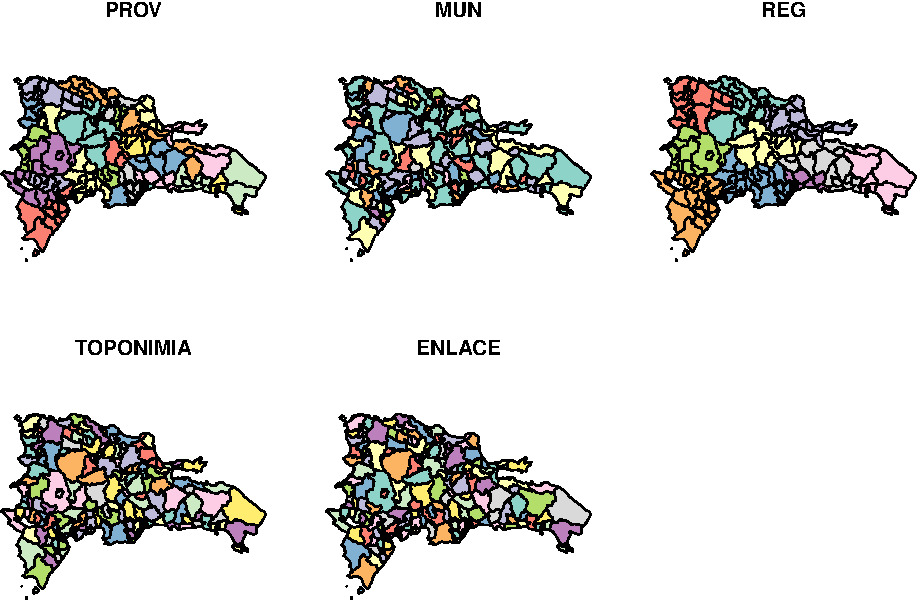
\includegraphics[width=1\linewidth]{img/unnamed-chunk-2-1}

\begin{Shaded}
\begin{Highlighting}[]

\CommentTok{# Carga los datos del censo 2010}
\NormalTok{vivpersgeom_sf <-}\StringTok{ }\KeywordTok{readRDS}\NormalTok{(}\StringTok{'data/vivpersgeom_sf.RDS'}\NormalTok{)}
\NormalTok{censo <-}\StringTok{ }\NormalTok{vivpersgeom_sf }\OperatorTok\StringTok{ }\KeywordTok{select}\NormalTok{(}\KeywordTok{matches}\NormalTok{(}\StringTok{'ENLACE|TOPONIMIA|Población total|Condición de ocupación|Nivel Educativo|Dificultad para Caminar o subir escalones: Si|Asiste o asistió a la escuela: Nunca asistió'))}

\StringTok{censo <- censo %>% mutate("Cantviv"=`Condición de ocupación: Ocupada con personas presentes`+ `Condición de ocupación: Desocupada`)}

\StringTok{censo <- censo %>% mutate("PorcPersD"= `Dificultad para Caminar o subir escalones: Si`/`Población total` * 100)}

\StringTok{censo <- censo %>% mutate("PorcPersD_log"= log(censo$PorcPersD))}

\StringTok{structure(censo)}
\StringTok{## Simple feature collection with 155 features and 14 fields}
\StringTok{## geometry type:  MULTIPOLYGON}
\StringTok{## dimension:      XY}
\StringTok{## bbox:           xmin: -72.01147 ymin: 17.47033 xmax: -68.32354 ymax: 19.93211}
\StringTok{## epsg (SRID):    4326}
\StringTok{## proj4string:    +proj=longlat +datum=WGS84 +no_defs}
\StringTok{## First 10 features:}
\StringTok{##                  TOPONIMIA ENLACE}
\StringTok{## 1  SANTO DOMINGO DE GUZMÁN 100101}
\StringTok{## 2                     AZUA 050201}
\StringTok{## 3              LAS CHARCAS 050202}
\StringTok{## 4     LAS YAYAS DE VIAJAMA 050203}
\StringTok{## 5          PADRE LAS CASAS 050204}
\StringTok{## 6                  PERALTA 050205}
\StringTok{## 7             SABANA YEGUA 050206}
\StringTok{## 8             PUEBLO VIEJO 050207}
\StringTok{## 9            TÁBARA ARRIBA 050208}
\StringTok{## 10                GUAYABAL 050209}
\StringTok{##    Condición de ocupación: Ocupada con personas presentes}
\StringTok{## 1                                                  288362}
\StringTok{## 2                                                   22797}
\StringTok{## 3                                                    3147}
\StringTok{## 4                                                    4807}
\StringTok{## 5                                                    5243}
\StringTok{## 6                                                    3144}
\StringTok{## 7                                                    4828}
\StringTok{## 8                                                    2689}
\StringTok{## 9                                                    4108}
\StringTok{## 10                                                   1386}
\StringTok{##    Condición de ocupación: Desocupada Población total}
\StringTok{## 1                               42200          965040}
\StringTok{## 2                                1920           91345}
\StringTok{## 3                                 944           11243}
\StringTok{## 4                                 798           17620}
\StringTok{## 5                                1345           20041}
\StringTok{## 6                                 446           15257}
\StringTok{## 7                                 594           19020}
\StringTok{## 8                                 208           11235}
\StringTok{## 9                                 426           17647}
\StringTok{## 10                                464            5263}
\StringTok{##    Dificultad para Caminar o subir escalones: Si}
\StringTok{## 1                                          31271}
\StringTok{## 2                                           2616}
\StringTok{## 3                                            323}
\StringTok{## 4                                            770}
\StringTok{## 5                                            804}
\StringTok{## 6                                            320}
\StringTok{## 7                                            675}
\StringTok{## 8                                            266}
\StringTok{## 9                                            437}
\StringTok{## 10                                           234}
\StringTok{##    Asiste o asistió a la escuela: Nunca asistió}
\StringTok{## 1                                         45138}
\StringTok{## 2                                         12617}
\StringTok{## 3                                          2329}
\StringTok{## 4                                          3442}
\StringTok{## 5                                          4336}
\StringTok{## 6                                          3528}
\StringTok{## 7                                          2813}
\StringTok{## 8                                          1629}
\StringTok{## 9                                          3860}
\StringTok{## 10                                          909}
\StringTok{##    Nivel educativo más alto al que asistió: Preprimaria}
\StringTok{## 1                                                 73199}
\StringTok{## 2                                                  7718}
\StringTok{## 3                                                   965}
\StringTok{## 4                                                  1400}
\StringTok{## 5                                                  2027}
\StringTok{## 6                                                  1360}
\StringTok{## 7                                                  1079}
\StringTok{## 8                                                   961}
\StringTok{## 9                                                  1344}
\StringTok{## 10                                                  240}
\StringTok{##    Nivel educativo más alto al que asistió: Primaria o básica}
\StringTok{## 1                                                      290061}
\StringTok{## 2                                                       37701}
\StringTok{## 3                                                        5361}
\StringTok{## 4                                                        8439}
\StringTok{## 5                                                        8458}
\StringTok{## 6                                                        5736}
\StringTok{## 7                                                        9246}
\StringTok{## 8                                                        5270}
\StringTok{## 9                                                        7916}
\StringTok{## 10                                                       2458}
\StringTok{##    Nivel educativo más alto al que asistió: Secundaria o media}
\StringTok{## 1                                                       248102}
\StringTok{## 2                                                        19003}
\StringTok{## 3                                                         1616}
\StringTok{## 4                                                         2757}
\StringTok{## 5                                                         3104}
\StringTok{## 6                                                         2823}
\StringTok{## 7                                                         3676}
\StringTok{## 8                                                         2133}
\StringTok{## 9                                                         2869}
\StringTok{## 10                                                         924}
\StringTok{##    Nivel educativo más alto al que asistió: Universitaria o superior}
\StringTok{## 1                                                             257590}
\StringTok{## 2                                                               8601}
\StringTok{## 3                                                                204}
\StringTok{## 4                                                                541}
\StringTok{## 5                                                               1075}
\StringTok{## 6                                                               1020}
\StringTok{## 7                                                               1048}
\StringTok{## 8                                                                484}
\StringTok{## 9                                                                602}
\StringTok{## 10                                                               479}
\StringTok{##                              geom Cantviv PorcPersD PorcPersD_log}
\StringTok{## 1  MULTIPOLYGON (((-69.89794 1...  330562  3.240384     1.1756918}
\StringTok{## 2  MULTIPOLYGON (((-70.71457 1...   24717  2.863868     1.0521731}
\StringTok{## 3  MULTIPOLYGON (((-70.50185 1...    4091  2.872899     1.0553215}
\StringTok{## 4  MULTIPOLYGON (((-70.85774 1...    5605  4.370034     1.4747708}
\StringTok{## 5  MULTIPOLYGON (((-70.77551 1...    6588  4.011776     1.3892340}
\StringTok{## 6  MULTIPOLYGON (((-70.73131 1...    3590  2.097398     0.7406975}
\StringTok{## 7  MULTIPOLYGON (((-70.83014 1...    5422  3.548896     1.2666365}
\StringTok{## 8  MULTIPOLYGON (((-70.79387 1...    2897  2.367601     0.8618773}
\StringTok{## 9  MULTIPOLYGON (((-70.83352 1...    4534  2.476342     0.9067823}
\StringTok{## 10 MULTIPOLYGON (((-70.68664 1...    1850  4.446133     1.4920348}

\StringTok{# Aseguro se trabaja con el mismo sistema de coordenadas}
\StringTok{censoT = st_transform(censo, crs=32619)  }

\StringTok{# Aseguro la relacion entre los archivos con el campo ENLACE y TOPONIMIA}
\StringTok{match(censoT$ENLACE, muni.sf$ENLACE)}
\StringTok{##   [1]   1   2   3   4   5   6   7   8   9  10  11  12  13  14  15  16  17}
\StringTok{##  [18]  18  19  20  21  22  23  24  25  26  27  28  29  30  31  32  33  34}
\StringTok{##  [35]  35  36  37  38  39  40  41  42  43  44  45  46  47  48  49  50  51}
\StringTok{##  [52]  52  53  54  55  56  57  58  59  60  61  62  63  64  65  66  67  68}
\StringTok{##  [69]  69  70  71  72  73  74  75  76  77  78  79  80  81  82  83  84  85}
\StringTok{##  [86]  86  87  88  89  90  91  92  93  94  95  96  97  98  99 100 101 102}
\StringTok{## [103] 103 104 105 106 107 108 109 110 111 112 113 114 115 116 117 118 119}
\StringTok{## [120] 120 121 122 123 124 125 126 127 128 129 130 131 132 133 134 135 136}
\StringTok{## [137] 137 138 139 140 141 142 143 144 145 146 147 148 149 150 151 152 153}
\StringTok{## [154] 154 155}
\StringTok{match(censoT$TOPONIMIA, muni.sf$TOPONIMIA)}
\StringTok{##   [1]   1   2   3   4   5   6   7   8   9  10  11  12  13  14  15  16  17}
\StringTok{##  [18]  18  19  20  21  22  23  24  25  26  27  28  29  30  31  32  33  34}
\StringTok{##  [35]  35  36  37  38  39  40  41  42  43  44  45  46  47  48  49  50  51}
\StringTok{##  [52]  52  53  54  55  56  57  58  59  60  61  62  63  64  65  66  67  68}
\StringTok{##  [69]  69  70  71  72  73  74  75  76  77  78  79  80  81  82  83  84  85}
\StringTok{##  [86]  86  87  88  89  90  91  92  93  94  95  96  97  98  99 100 101 102}
\StringTok{## [103] 103 104 105 106 107 108 109 110 111 112 113 114 115 116 117 118 119}
\StringTok{## [120] 120 121 122 123 124 125 126 127 128 129 130 131 132 133 134 135 136}
\StringTok{## [137] 137 138 139 140 141 142 143 144 145 146 147 148 149 150 151 152 153}
\StringTok{## [154] 154 155}
\end{Highlighting}
\end{Shaded}

\subsection{Analisis Exploratorio
ESDA}\label{analisis-exploratorio-esda}

\begin{Shaded}
\begin{Highlighting}[]
\KeywordTok{nrow}\NormalTok{(censoT)}
\NormalTok{## [1] 155}
\KeywordTok{summary}\NormalTok{(censoT}\OperatorTok{$}\StringTok{`}\DataTypeTok{Dificultad para Caminar o subir escalones: Si}\StringTok{`}\NormalTok{)}
\NormalTok{##    Min. 1st Qu.  Median    Mean 3rd Qu.    Max. }
\NormalTok{##     113     443     902    2114    1819   31271}
\NormalTok{Dificam <-}\StringTok{ }\NormalTok{censoT}\OperatorTok{$}\StringTok{`}\DataTypeTok{Dificultad para Caminar o subir escalones: Si}\StringTok{`}
\KeywordTok{hist}\NormalTok{(Dificam)}
\end{Highlighting}
\end{Shaded}

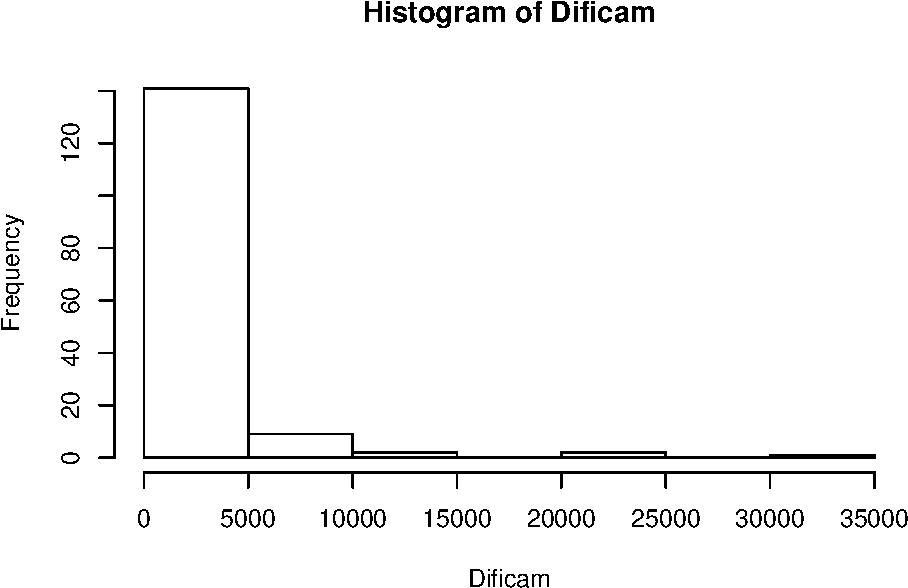
\includegraphics[width=1\linewidth]{img/unnamed-chunk-3-1}

\begin{Shaded}
\begin{Highlighting}[]
\KeywordTok{hist}\NormalTok{(}\KeywordTok{log}\NormalTok{(Dificam))}
\end{Highlighting}
\end{Shaded}

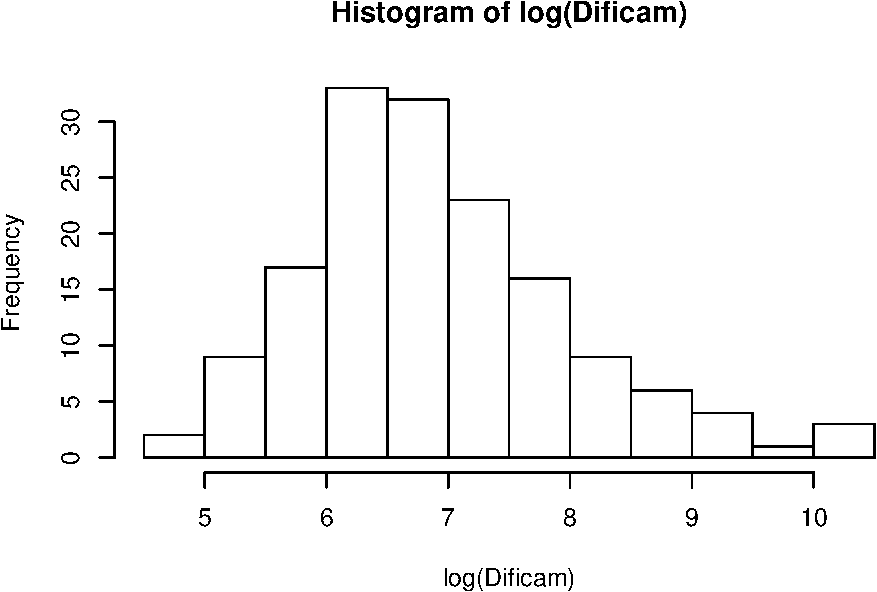
\includegraphics[width=1\linewidth]{img/unnamed-chunk-3-2}

\begin{Shaded}
\begin{Highlighting}[]
\KeywordTok{shapiro.test}\NormalTok{(Dificam)}
\NormalTok{## }
\NormalTok{##  Shapiro-Wilk normality test}
\NormalTok{## }
\NormalTok{## data:  Dificam}
\NormalTok{## W = 0.44601, p-value < 2.2e-16}
\KeywordTok{shapiro.test}\NormalTok{(}\KeywordTok{log}\NormalTok{(Dificam))}
\NormalTok{## }
\NormalTok{##  Shapiro-Wilk normality test}
\NormalTok{## }
\NormalTok{## data:  log(Dificam)}
\NormalTok{## W = 0.96842, p-value = 0.001267}
\KeywordTok{qqnorm}\NormalTok{(Dificam)}
\end{Highlighting}
\end{Shaded}

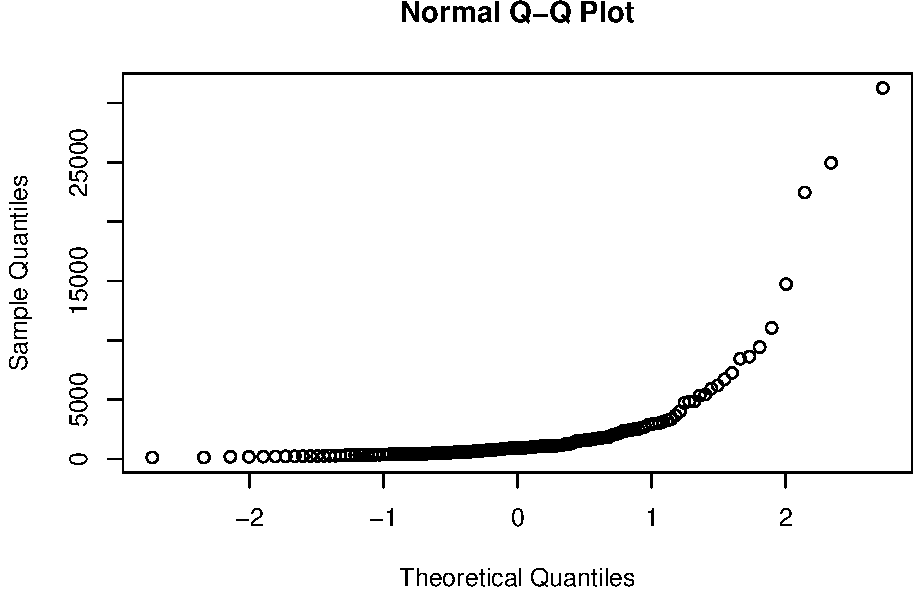
\includegraphics[width=1\linewidth]{img/unnamed-chunk-3-3}

\begin{Shaded}
\begin{Highlighting}[]
\KeywordTok{qqnorm}\NormalTok{(}\KeywordTok{log}\NormalTok{(Dificam))}
\end{Highlighting}
\end{Shaded}

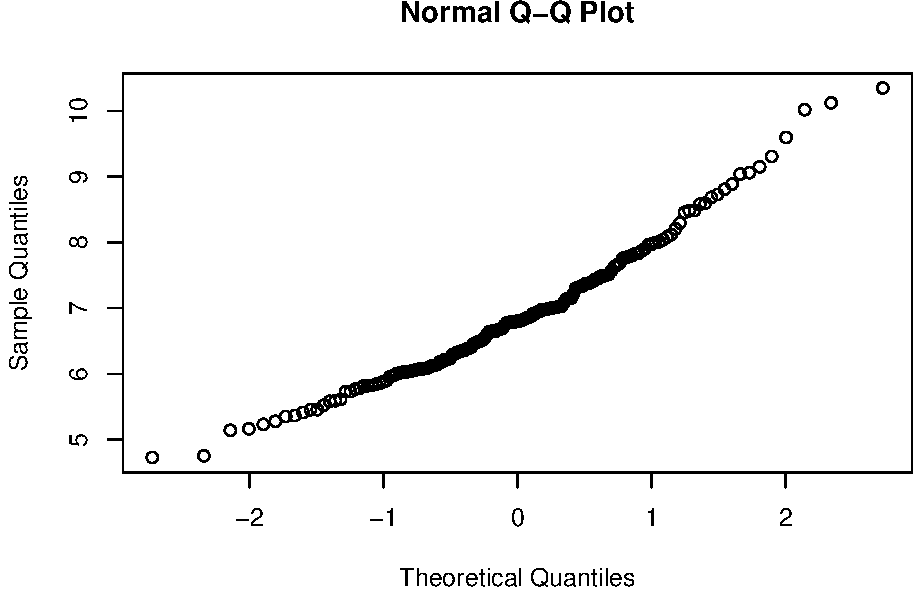
\includegraphics[width=1\linewidth]{img/unnamed-chunk-3-4}

\begin{Shaded}
\begin{Highlighting}[]
\NormalTok{Dificam_log <-}\StringTok{ }\KeywordTok{log}\NormalTok{(Dificam)}
\NormalTok{censoT <-}\StringTok{ }\NormalTok{censoT }\OperatorTok\StringTok{ }\KeywordTok{mutate}\NormalTok{(}\StringTok{"Dificam_log"}\NormalTok{ =}\StringTok{ }\KeywordTok{log}\NormalTok{(Dificam))}
\end{Highlighting}
\end{Shaded}

\subsection{Analisis de Vecindad}\label{analisis-de-vecindad}

\begin{Shaded}
\begin{Highlighting}[]
\CommentTok{# Vecindad por Contiguidad: Se crea objeto de vecindad con el criterio donde todos son vecinos}
\NormalTok{censoT.sp <-}\StringTok{ }\KeywordTok{as_Spatial}\NormalTok{(censoT)}
\NormalTok{censoT.np <-}\StringTok{ }\KeywordTok{poly2nb}\NormalTok{(censoT.sp, }\DataTypeTok{queen =} \OtherTok{TRUE}\NormalTok{) }
\KeywordTok{summary}\NormalTok{(censoT.np)}
\NormalTok{## Neighbour list object:}
\NormalTok{## Number of regions: 155 }
\NormalTok{## Number of nonzero links: 804 }
\NormalTok{## Percentage nonzero weights: 3.346514 }
\NormalTok{## Average number of links: 5.187097 }
\NormalTok{## Link number distribution:}
\NormalTok{## }
\NormalTok{##  1  2  3  4  5  6  7  8  9 10 11 12 14 }
\NormalTok{##  1 10 20 34 33 22 13 13  4  1  1  2  1 }
\NormalTok{## 1 least connected region:}
\NormalTok{## 107 with 1 link}
\NormalTok{## 1 most connected region:}
\NormalTok{## 63 with 14 links}

\CommentTok{# Evaluación de cardinalidad}
\KeywordTok{card}\NormalTok{(censoT.np)   }
\NormalTok{##   [1]  4  6  3  6  7  6  3  2  6  5  5  7  5  8  4  3  4  7  4  3  5  6  4}
\NormalTok{##  [24]  4  4  8  5  5  4  6  4  5 12  4  5  6  7  4  5  3  3  4  4  6  5  8}
\NormalTok{##  [47]  3 10  3  7  3  2  3  3  5  7  8  5  2  4  5  3 14  8  7  3  6  2  5}
\NormalTok{##  [70]  4  5  4  8  5  2  3  5  2  6  3  8  7  4  5  6  4  5  4  2  7  4  4}
\NormalTok{##  [93]  2  7  2  9  3  3  5  6  5  2  6 11  4  8  1  7  5  4  6  5  5  5  4}
\NormalTok{## [116]  9  6  7  4 12  5  5  4  8  4  3  5  4  9  4  3  8  6  5  9  4  6  8}
\NormalTok{## [139]  7  6  8  4  6  6  4  8  3  6  5  4  6  4  5  5  5}
\KeywordTok{sapply}\NormalTok{(censoT.np, }\ControlFlowTok{function}\NormalTok{(x) x)}
\NormalTok{## [[1]]}
\NormalTok{## [1] 149 150 151 154}
\NormalTok{## }
\NormalTok{## [[2]]}
\NormalTok{## [1]  6  7  8  9 11 27}
\NormalTok{## }
\NormalTok{## [[3]]}
\NormalTok{## [1]  11  79 146}
\NormalTok{## }
\NormalTok{## [[4]]}
\NormalTok{## [1]   5   6   9  14  21 104}
\NormalTok{## }
\NormalTok{## [[5]]}
\NormalTok{## [1]   4   6  10  64  65 104 105}
\NormalTok{## }
\NormalTok{## [[6]]}
\NormalTok{## [1]  2  4  5  9 10 11}
\NormalTok{## }
\NormalTok{## [[7]]}
\NormalTok{## [1] 2 8 9}
\NormalTok{## }
\NormalTok{## [[8]]}
\NormalTok{## [1] 2 7}
\NormalTok{## }
\NormalTok{## [[9]]}
\NormalTok{## [1]  2  4  6  7 21 27}
\NormalTok{## }
\NormalTok{## [[10]]}
\NormalTok{## [1]   5   6  11  64 146}
\NormalTok{## }
\NormalTok{## [[11]]}
\NormalTok{## [1]   2   3   6  10 146}
\NormalTok{## }
\NormalTok{## [[12]]}
\NormalTok{## [1]  13  14  15  56  57 106 109}
\NormalTok{## }
\NormalTok{## [[13]]}
\NormalTok{## [1]  12  14  56  57 109}
\NormalTok{## }
\NormalTok{## [[14]]}
\NormalTok{## [1]   4  12  13  21  22  56 104 109}
\NormalTok{## }
\NormalTok{## [[15]]}
\NormalTok{## [1]  12  16  57 106}
\NormalTok{## }
\NormalTok{## [[16]]}
\NormalTok{## [1]  15  55 106}
\NormalTok{## }
\NormalTok{## [[17]]}
\NormalTok{## [1] 18 23 24 26}
\NormalTok{## }
\NormalTok{## [[18]]}
\NormalTok{## [1] 17 22 23 24 25 26 56}
\NormalTok{## }
\NormalTok{## [[19]]}
\NormalTok{## [1] 20 26 77 78}
\NormalTok{## }
\NormalTok{## [[20]]}
\NormalTok{## [1] 19 23 26}
\NormalTok{## }
\NormalTok{## [[21]]}
\NormalTok{## [1]  4  9 14 22 27}
\NormalTok{## }
\NormalTok{## [[22]]}
\NormalTok{## [1] 14 18 21 24 27 56}
\NormalTok{## }
\NormalTok{## [[23]]}
\NormalTok{## [1] 17 18 20 26}
\NormalTok{## }
\NormalTok{## [[24]]}
\NormalTok{## [1] 17 18 22 27}
\NormalTok{## }
\NormalTok{## [[25]]}
\NormalTok{## [1] 18 26 56 57}
\NormalTok{## }
\NormalTok{## [[26]]}
\NormalTok{## [1] 17 18 19 20 23 25 57 77}
\NormalTok{## }
\NormalTok{## [[27]]}
\NormalTok{## [1]  2  9 21 22 24}
\NormalTok{## }
\NormalTok{## [[28]]}
\NormalTok{## [1] 29 30 71 74 75}
\NormalTok{## }
\NormalTok{## [[29]]}
\NormalTok{## [1] 28 30 31 32}
\NormalTok{## }
\NormalTok{## [[30]]}
\NormalTok{## [1]  28  29  32  73  74 129}
\NormalTok{## }
\NormalTok{## [[31]]}
\NormalTok{## [1]  29  32  44 130}
\NormalTok{## }
\NormalTok{## [[32]]}
\NormalTok{## [1]  29  30  31 129 130}
\NormalTok{## }
\NormalTok{## [[33]]}
\NormalTok{##  [1]  35  36  38  50  63  67  69  70  90  91  92 118}
\NormalTok{## }
\NormalTok{## [[34]]}
\NormalTok{## [1] 37 67 69 94}
\NormalTok{## }
\NormalTok{## [[35]]}
\NormalTok{## [1] 33 36 37 39 69}
\NormalTok{## }
\NormalTok{## [[36]]}
\NormalTok{## [1]  33  35  38  39 116 119}
\NormalTok{## }
\NormalTok{## [[37]]}
\NormalTok{## [1]  34  35  39  69  94 117 140}
\NormalTok{## }
\NormalTok{## [[38]]}
\NormalTok{## [1]  33  36 118 119}
\NormalTok{## }
\NormalTok{## [[39]]}
\NormalTok{## [1]  35  36  37 116 117}
\NormalTok{## }
\NormalTok{## [[40]]}
\NormalTok{## [1]  41  42 108}
\NormalTok{## }
\NormalTok{## [[41]]}
\NormalTok{## [1]  40  44 108}
\NormalTok{## }
\NormalTok{## [[42]]}
\NormalTok{## [1]  40  43  45 108}
\NormalTok{## }
\NormalTok{## [[43]]}
\NormalTok{## [1] 42 45 54 55}
\NormalTok{## }
\NormalTok{## [[44]]}
\NormalTok{## [1]  31  41 104 108 129 130}
\NormalTok{## }
\NormalTok{## [[45]]}
\NormalTok{## [1]  42  43  55 106 108}
\NormalTok{## }
\NormalTok{## [[46]]}
\NormalTok{## [1]  47  58  61 112 113 143 144 145}
\NormalTok{## }
\NormalTok{## [[47]]}
\NormalTok{## [1]  46  58 144}
\NormalTok{## }
\NormalTok{## [[48]]}
\NormalTok{##  [1]  49  50  51  63  81  87  90 123 125 127}
\NormalTok{## }
\NormalTok{## [[49]]}
\NormalTok{## [1] 48 63 90}
\NormalTok{## }
\NormalTok{## [[50]]}
\NormalTok{## [1] 33 48 51 70 87 90 91}
\NormalTok{## }
\NormalTok{## [[51]]}
\NormalTok{## [1] 48 50 87}
\NormalTok{## }
\NormalTok{## [[52]]}
\NormalTok{## [1] 53 54}
\NormalTok{## }
\NormalTok{## [[53]]}
\NormalTok{## [1] 52 57 77}
\NormalTok{## }
\NormalTok{## [[54]]}
\NormalTok{## [1] 43 52 55}
\NormalTok{## }
\NormalTok{## [[55]]}
\NormalTok{## [1]  16  43  45  54 106}
\NormalTok{## }
\NormalTok{## [[56]]}
\NormalTok{## [1] 12 13 14 18 22 25 57}
\NormalTok{## }
\NormalTok{## [[57]]}
\NormalTok{## [1] 12 13 15 25 26 53 56 77}
\NormalTok{## }
\NormalTok{## [[58]]}
\NormalTok{## [1] 46 47 59 60 61}
\NormalTok{## }
\NormalTok{## [[59]]}
\NormalTok{## [1] 58 60}
\NormalTok{## }
\NormalTok{## [[60]]}
\NormalTok{## [1] 58 59 61 62}
\NormalTok{## }
\NormalTok{## [[61]]}
\NormalTok{## [1]  46  58  60  62 112}
\NormalTok{## }
\NormalTok{## [[62]]}
\NormalTok{## [1]  60  61 112}
\NormalTok{## }
\NormalTok{## [[63]]}
\NormalTok{##  [1]  33  48  49  64  65  66  90  92 118 120 122 127 128 135}
\NormalTok{## }
\NormalTok{## [[64]]}
\NormalTok{## [1]   5  10  63  65 135 146 147 148}
\NormalTok{## }
\NormalTok{## [[65]]}
\NormalTok{## [1]   5  63  64 105 122 124 135}
\NormalTok{## }
\NormalTok{## [[66]]}
\NormalTok{## [1]  63 118 135}
\NormalTok{## }
\NormalTok{## [[67]]}
\NormalTok{## [1] 33 34 68 69 70 94}
\NormalTok{## }
\NormalTok{## [[68]]}
\NormalTok{## [1] 67 70}
\NormalTok{## }
\NormalTok{## [[69]]}
\NormalTok{## [1] 33 34 35 37 67}
\NormalTok{## }
\NormalTok{## [[70]]}
\NormalTok{## [1] 33 50 67 68}
\NormalTok{## }
\NormalTok{## [[71]]}
\NormalTok{## [1] 28 72 74 75 76}
\NormalTok{## }
\NormalTok{## [[72]]}
\NormalTok{## [1] 71 73 74 76}
\NormalTok{## }
\NormalTok{## [[73]]}
\NormalTok{## [1]  30  72  74  76  88 129 132 134}
\NormalTok{## }
\NormalTok{## [[74]]}
\NormalTok{## [1] 28 30 71 72 73}
\NormalTok{## }
\NormalTok{## [[75]]}
\NormalTok{## [1] 28 71}
\NormalTok{## }
\NormalTok{## [[76]]}
\NormalTok{## [1] 71 72 73}
\NormalTok{## }
\NormalTok{## [[77]]}
\NormalTok{## [1] 19 26 53 57 78}
\NormalTok{## }
\NormalTok{## [[78]]}
\NormalTok{## [1] 19 77}
\NormalTok{## }
\NormalTok{## [[79]]}
\NormalTok{## [1]   3  80  99 101 103 146}
\NormalTok{## }
\NormalTok{## [[80]]}
\NormalTok{## [1]  79  97 101}
\NormalTok{## }
\NormalTok{## [[81]]}
\NormalTok{## [1]  48  82  84  86  87  89 120 125}
\NormalTok{## }
\NormalTok{## [[82]]}
\NormalTok{## [1]  81  83  84 120 121 126 133}
\NormalTok{## }
\NormalTok{## [[83]]}
\NormalTok{## [1]  82  84  85 133}
\NormalTok{## }
\NormalTok{## [[84]]}
\NormalTok{## [1] 81 82 83 85 86}
\NormalTok{## }
\NormalTok{## [[85]]}
\NormalTok{## [1]  83  84  86  88 133 134}
\NormalTok{## }
\NormalTok{## [[86]]}
\NormalTok{## [1] 81 84 85 88}
\NormalTok{## }
\NormalTok{## [[87]]}
\NormalTok{## [1] 48 50 51 81 89}
\NormalTok{## }
\NormalTok{## [[88]]}
\NormalTok{## [1]  73  85  86 134}
\NormalTok{## }
\NormalTok{## [[89]]}
\NormalTok{## [1] 81 87}
\NormalTok{## }
\NormalTok{## [[90]]}
\NormalTok{## [1] 33 48 49 50 63 91 92}
\NormalTok{## }
\NormalTok{## [[91]]}
\NormalTok{## [1] 33 50 90 92}
\NormalTok{## }
\NormalTok{## [[92]]}
\NormalTok{## [1] 33 63 90 91}
\NormalTok{## }
\NormalTok{## [[93]]}
\NormalTok{## [1] 94 95}
\NormalTok{## }
\NormalTok{## [[94]]}
\NormalTok{## [1]  34  37  67  93  95 140 144}
\NormalTok{## }
\NormalTok{## [[95]]}
\NormalTok{## [1] 93 94}
\NormalTok{## }
\NormalTok{## [[96]]}
\NormalTok{## [1]  97  98  99 100 101 102 150 154 155}
\NormalTok{## }
\NormalTok{## [[97]]}
\NormalTok{## [1]  80  96 101}
\NormalTok{## }
\NormalTok{## [[98]]}
\NormalTok{## [1]  96 102 150}
\NormalTok{## }
\NormalTok{## [[99]]}
\NormalTok{## [1]  79  96 100 101 103}
\NormalTok{## }
\NormalTok{## [[100]]}
\NormalTok{## [1]  96  99 103 137 141 155}
\NormalTok{## }
\NormalTok{## [[101]]}
\NormalTok{## [1] 79 80 96 97 99}
\NormalTok{## }
\NormalTok{## [[102]]}
\NormalTok{## [1] 96 98}
\NormalTok{## }
\NormalTok{## [[103]]}
\NormalTok{## [1]  79  99 100 137 146 148}
\NormalTok{## }
\NormalTok{## [[104]]}
\NormalTok{##  [1]   4   5  14  44 105 106 107 108 109 124 129}
\NormalTok{## }
\NormalTok{## [[105]]}
\NormalTok{## [1]   5  65 104 124}
\NormalTok{## }
\NormalTok{## [[106]]}
\NormalTok{## [1]  12  15  16  45  55 104 108 109}
\NormalTok{## }
\NormalTok{## [[107]]}
\NormalTok{## [1] 104}
\NormalTok{## }
\NormalTok{## [[108]]}
\NormalTok{## [1]  40  41  42  44  45 104 106}
\NormalTok{## }
\NormalTok{## [[109]]}
\NormalTok{## [1]  12  13  14 104 106}
\NormalTok{## }
\NormalTok{## [[110]]}
\NormalTok{## [1] 112 113 114 115}
\NormalTok{## }
\NormalTok{## [[111]]}
\NormalTok{## [1] 114 115 139 143 152 153}
\NormalTok{## }
\NormalTok{## [[112]]}
\NormalTok{## [1]  46  61  62 110 113}
\NormalTok{## }
\NormalTok{## [[113]]}
\NormalTok{## [1]  46 110 112 114 143}
\NormalTok{## }
\NormalTok{## [[114]]}
\NormalTok{## [1] 110 111 113 115 143}
\NormalTok{## }
\NormalTok{## [[115]]}
\NormalTok{## [1] 110 111 114 152}
\NormalTok{## }
\NormalTok{## [[116]]}
\NormalTok{## [1]  36  39 117 118 119 135 136 141 142}
\NormalTok{## }
\NormalTok{## [[117]]}
\NormalTok{## [1]  37  39 116 138 140 142}
\NormalTok{## }
\NormalTok{## [[118]]}
\NormalTok{## [1]  33  38  63  66 116 119 135}
\NormalTok{## }
\NormalTok{## [[119]]}
\NormalTok{## [1]  36  38 116 118}
\NormalTok{## }
\NormalTok{## [[120]]}
\NormalTok{##  [1]  63  81  82 121 122 123 124 125 126 127 128 132}
\NormalTok{## }
\NormalTok{## [[121]]}
\NormalTok{## [1]  82 120 126 132 133}
\NormalTok{## }
\NormalTok{## [[122]]}
\NormalTok{## [1]  63  65 120 124 128}
\NormalTok{## }
\NormalTok{## [[123]]}
\NormalTok{## [1]  48 120 125 127}
\NormalTok{## }
\NormalTok{## [[124]]}
\NormalTok{## [1]  65 104 105 120 122 129 131 132}
\NormalTok{## }
\NormalTok{## [[125]]}
\NormalTok{## [1]  48  81 120 123}
\NormalTok{## }
\NormalTok{## [[126]]}
\NormalTok{## [1]  82 120 121}
\NormalTok{## }
\NormalTok{## [[127]]}
\NormalTok{## [1]  48  63 120 123 128}
\NormalTok{## }
\NormalTok{## [[128]]}
\NormalTok{## [1]  63 120 122 127}
\NormalTok{## }
\NormalTok{## [[129]]}
\NormalTok{## [1]  30  32  44  73 104 124 130 131 132}
\NormalTok{## }
\NormalTok{## [[130]]}
\NormalTok{## [1]  31  32  44 129}
\NormalTok{## }
\NormalTok{## [[131]]}
\NormalTok{## [1] 124 129 132}
\NormalTok{## }
\NormalTok{## [[132]]}
\NormalTok{## [1]  73 120 121 124 129 131 133 134}
\NormalTok{## }
\NormalTok{## [[133]]}
\NormalTok{## [1]  82  83  85 121 132 134}
\NormalTok{## }
\NormalTok{## [[134]]}
\NormalTok{## [1]  73  85  88 132 133}
\NormalTok{## }
\NormalTok{## [[135]]}
\NormalTok{## [1]  63  64  65  66 116 118 136 137 148}
\NormalTok{## }
\NormalTok{## [[136]]}
\NormalTok{## [1] 116 135 137 141}
\NormalTok{## }
\NormalTok{## [[137]]}
\NormalTok{## [1] 100 103 135 136 141 148}
\NormalTok{## }
\NormalTok{## [[138]]}
\NormalTok{## [1] 117 139 140 141 142 149 151 153}
\NormalTok{## }
\NormalTok{## [[139]]}
\NormalTok{## [1] 111 138 140 143 144 145 153}
\NormalTok{## }
\NormalTok{## [[140]]}
\NormalTok{## [1]  37  94 117 138 139 144}
\NormalTok{## }
\NormalTok{## [[141]]}
\NormalTok{## [1] 100 116 136 137 138 142 151 155}
\NormalTok{## }
\NormalTok{## [[142]]}
\NormalTok{## [1] 116 117 138 141}
\NormalTok{## }
\NormalTok{## [[143]]}
\NormalTok{## [1]  46 111 113 114 139 145}
\NormalTok{## }
\NormalTok{## [[144]]}
\NormalTok{## [1]  46  47  94 139 140 145}
\NormalTok{## }
\NormalTok{## [[145]]}
\NormalTok{## [1]  46 139 143 144}
\NormalTok{## }
\NormalTok{## [[146]]}
\NormalTok{## [1]   3  10  11  64  79 103 147 148}
\NormalTok{## }
\NormalTok{## [[147]]}
\NormalTok{## [1]  64 146 148}
\NormalTok{## }
\NormalTok{## [[148]]}
\NormalTok{## [1]  64 103 135 137 146 147}
\NormalTok{## }
\NormalTok{## [[149]]}
\NormalTok{## [1]   1 138 151 152 153}
\NormalTok{## }
\NormalTok{## [[150]]}
\NormalTok{## [1]   1  96  98 154}
\NormalTok{## }
\NormalTok{## [[151]]}
\NormalTok{## [1]   1 138 141 149 154 155}
\NormalTok{## }
\NormalTok{## [[152]]}
\NormalTok{## [1] 111 115 149 153}
\NormalTok{## }
\NormalTok{## [[153]]}
\NormalTok{## [1] 111 138 139 149 152}
\NormalTok{## }
\NormalTok{## [[154]]}
\NormalTok{## [1]   1  96 150 151 155}
\NormalTok{## }
\NormalTok{## [[155]]}
\NormalTok{## [1]  96 100 141 151 154}

\CommentTok{#resultado: Es simetrico}
\KeywordTok{is.symmetric.nb}\NormalTok{(censoT.np)   }
\NormalTok{## [1] TRUE}

\KeywordTok{plot}\NormalTok{(censoT.sp, }\DataTypeTok{border=}\StringTok{"red"}\NormalTok{, }\DataTypeTok{lwd=}\DecValTok{1}\NormalTok{)}
\KeywordTok{plot}\NormalTok{(censoT.np, }\KeywordTok{coordinates}\NormalTok{(censoT.sp), }\DataTypeTok{add=}\NormalTok{T)}
\end{Highlighting}
\end{Shaded}

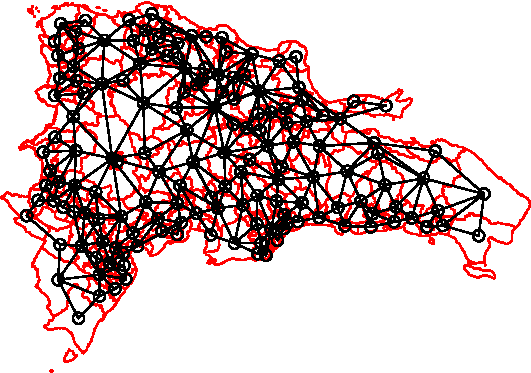
\includegraphics[width=1\linewidth]{img/unnamed-chunk-4-1}

\begin{Shaded}
\begin{Highlighting}[]

\CommentTok{# Vecindad por numero de vecinos: Se crea objeto de vecindad donde cada municipio tenga solo un vecino próximo}
\NormalTok{coords <-}\StringTok{ }\KeywordTok{coordinates}\NormalTok{(censoT.sp)}
\NormalTok{ident <-}\StringTok{ }\KeywordTok{row.names}\NormalTok{(censoT.sp)}
\NormalTok{censoT.np.k1 <-}\StringTok{ }\KeywordTok{knn2nb}\NormalTok{(}\KeywordTok{knearneigh}\NormalTok{(coords,}\DataTypeTok{k=}\DecValTok{1}\NormalTok{), }\DataTypeTok{row.names =}\NormalTok{ ident)}
\NormalTok{censoT.np.k2 <-}\StringTok{ }\KeywordTok{knn2nb}\NormalTok{(}\KeywordTok{knearneigh}\NormalTok{(coords,}\DataTypeTok{k=}\DecValTok{2}\NormalTok{), }\DataTypeTok{row.names =}\NormalTok{ ident)}

\KeywordTok{is.symmetric.nb}\NormalTok{(censoT.np.k1)}
\NormalTok{## [1] FALSE}
\KeywordTok{is.symmetric.nb}\NormalTok{(censoT.np.k2)}
\NormalTok{## [1] FALSE}

\CommentTok{# Resultado: En ambos casos NO es simetrico}
\KeywordTok{plot}\NormalTok{(censoT.sp, }\DataTypeTok{border=}\StringTok{"red"}\NormalTok{, }\DataTypeTok{lwd=}\DecValTok{1}\NormalTok{)}
\KeywordTok{plot}\NormalTok{(censoT.np.k1, }\KeywordTok{coordinates}\NormalTok{(censoT.sp), }\DataTypeTok{add=}\NormalTok{T)}
\end{Highlighting}
\end{Shaded}

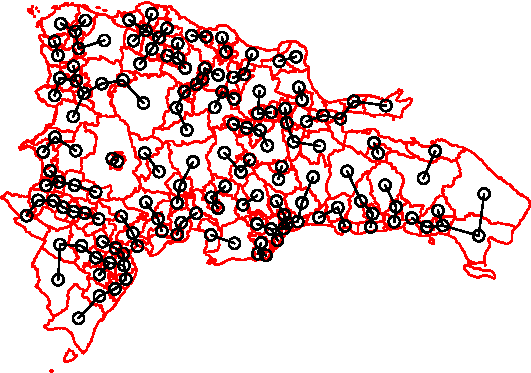
\includegraphics[width=1\linewidth]{img/unnamed-chunk-4-2}

\begin{Shaded}
\begin{Highlighting}[]

\KeywordTok{plot}\NormalTok{(censoT.sp, }\DataTypeTok{border=}\StringTok{"red"}\NormalTok{, }\DataTypeTok{lwd=}\DecValTok{1}\NormalTok{)}
\KeywordTok{plot}\NormalTok{(censoT.np.k2, }\KeywordTok{coordinates}\NormalTok{(censoT.sp), }\DataTypeTok{add=}\NormalTok{T)}
\end{Highlighting}
\end{Shaded}

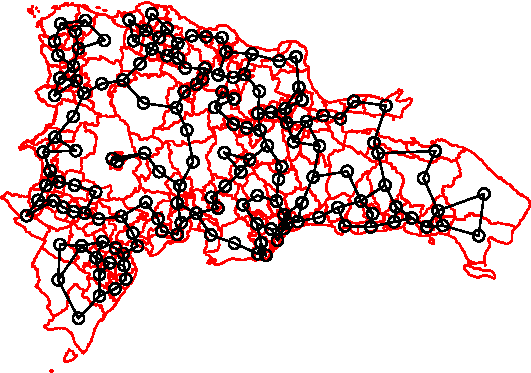
\includegraphics[width=1\linewidth]{img/unnamed-chunk-4-3}

\begin{Shaded}
\begin{Highlighting}[]

\CommentTok{# Determinamos la distancia máxima y mínima al vecino mas proximo usando k=1}
\NormalTok{dist <-}\StringTok{ }\KeywordTok{unlist}\NormalTok{(}\KeywordTok{nbdists}\NormalTok{(censoT.np.k1, coords))}
\KeywordTok{summary}\NormalTok{(dist)}
\NormalTok{##    Min. 1st Qu.  Median    Mean 3rd Qu.    Max. }
\NormalTok{##    4290    9657   11042   12320   13872   31017}
\KeywordTok{hist}\NormalTok{(dist)}
\end{Highlighting}
\end{Shaded}

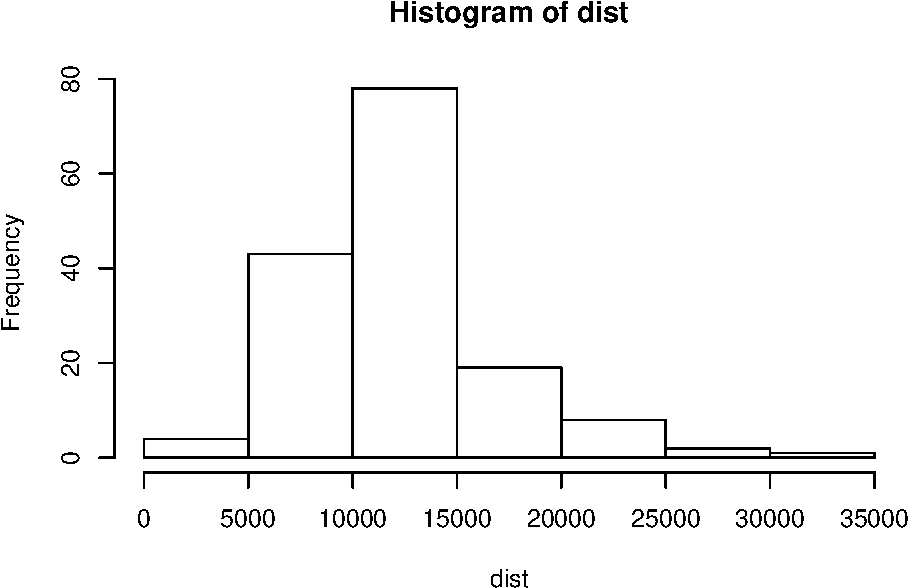
\includegraphics[width=1\linewidth]{img/unnamed-chunk-4-4}

\begin{Shaded}
\begin{Highlighting}[]
\KeywordTok{boxplot}\NormalTok{(dist)}
\end{Highlighting}
\end{Shaded}

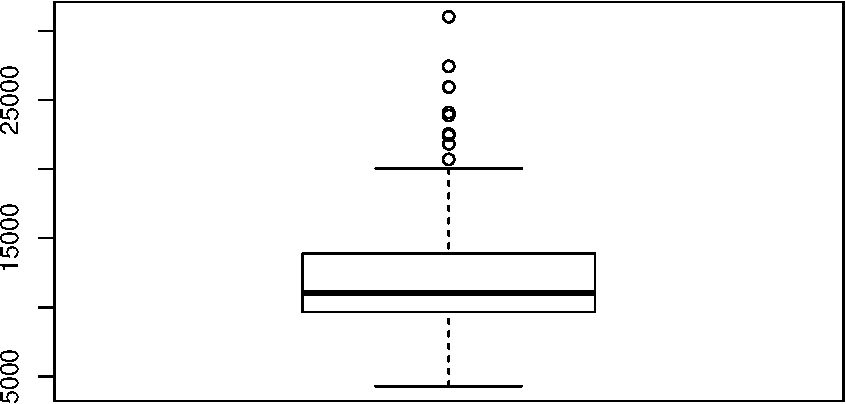
\includegraphics[width=1\linewidth]{img/unnamed-chunk-4-5}

\begin{Shaded}
\begin{Highlighting}[]
\KeywordTok{rownames}\NormalTok{(censoT) <-}\StringTok{ }\NormalTok{censoT}\OperatorTok{$}\NormalTok{TOPONIMIA}
\NormalTok{nb <-}\StringTok{ }\KeywordTok{poly2nb}\NormalTok{(censoT)}
\KeywordTok{summary}\NormalTok{(nb)}
\NormalTok{## Neighbour list object:}
\NormalTok{## Number of regions: 155 }
\NormalTok{## Number of nonzero links: 804 }
\NormalTok{## Percentage nonzero weights: 3.346514 }
\NormalTok{## Average number of links: 5.187097 }
\NormalTok{## Link number distribution:}
\NormalTok{## }
\NormalTok{##  1  2  3  4  5  6  7  8  9 10 11 12 14 }
\NormalTok{##  1 10 20 34 33 22 13 13  4  1  1  2  1 }
\NormalTok{## 1 least connected region:}
\NormalTok{## JUAN DE HERRERA with 1 link}
\NormalTok{## 1 most connected region:}
\NormalTok{## LA VEGA with 14 links}
\end{Highlighting}
\end{Shaded}

\subsection{Ponderadores espaciales (Construcción de objeto de
pesos)}\label{ponderadores-espaciales-construcciuxf3n-de-objeto-de-pesos}

\begin{Shaded}
\begin{Highlighting}[]
\CommentTok{# Estilo Weighted. Donde los pesos de las observaciones vecinas suman 1. Estandarización por fila}
\NormalTok{censo.w.w <-}\StringTok{ }\KeywordTok{nb2listw}\NormalTok{(nb)}
\NormalTok{censo.w.w}
\NormalTok{## Characteristics of weights list object:}
\NormalTok{## Neighbour list object:}
\NormalTok{## Number of regions: 155 }
\NormalTok{## Number of nonzero links: 804 }
\NormalTok{## Percentage nonzero weights: 3.346514 }
\NormalTok{## Average number of links: 5.187097 }
\NormalTok{## }
\NormalTok{## Weights style: W }
\NormalTok{## Weights constants summary:}
\NormalTok{##     n    nn  S0       S1       S2}
\NormalTok{## W 155 24025 155 65.94606 650.7687}

\CommentTok{# Estilo Binario. Donde los pesos son indicativos de la relación entre dos o mas observaciones.}
\NormalTok{censo.w.b <-}\StringTok{ }\KeywordTok{nb2listw}\NormalTok{(nb, }\DataTypeTok{style =} \StringTok{'B'}\NormalTok{)}
\NormalTok{censo.w.b}
\NormalTok{## Characteristics of weights list object:}
\NormalTok{## Neighbour list object:}
\NormalTok{## Number of regions: 155 }
\NormalTok{## Number of nonzero links: 804 }
\NormalTok{## Percentage nonzero weights: 3.346514 }
\NormalTok{## Average number of links: 5.187097 }
\NormalTok{## }
\NormalTok{## Weights style: B }
\NormalTok{## Weights constants summary:}
\NormalTok{##     n    nn  S0   S1    S2}
\NormalTok{## B 155 24025 804 1608 19520}
\end{Highlighting}
\end{Shaded}

\subsection{Autocorrelacion Espacial}\label{autocorrelacion-espacial}

\begin{Shaded}
\begin{Highlighting}[]
\CommentTok{# Prueba de Breuch-Pagan}
\NormalTok{coordsxy <-}\StringTok{ }\NormalTok{censoT }\OperatorTok
\StringTok{  }\KeywordTok{st_centroid}\NormalTok{() }\OperatorTok\StringTok{ }
\StringTok{     }\KeywordTok{mutate}\NormalTok{ (}\DataTypeTok{x=}\KeywordTok{unlist}\NormalTok{(}\KeywordTok{map}\NormalTok{(geom,}\DecValTok{1}\NormalTok{)),}
             \DataTypeTok{y=}\KeywordTok{unlist}\NormalTok{(}\KeywordTok{map}\NormalTok{(geom,}\DecValTok{2}\NormalTok{))) }\OperatorTok
\StringTok{  }\KeywordTok{st_drop_geometry}\NormalTok{() }\OperatorTok
\StringTok{  }\KeywordTok{select}\NormalTok{(ENLACE, x, y)}
\NormalTok{## Warning in st_centroid.sf(.): st_centroid assumes attributes are constant}
\NormalTok{## over geometries of x}
\NormalTok{coordsxy}
\NormalTok{##     ENLACE        x       y}
\NormalTok{## 1   100101 400576.8 2044091}
\NormalTok{## 2   050201 308829.1 2037708}
\NormalTok{## 3   050202 336675.2 2034232}
\NormalTok{## 4   050203 289007.6 2058192}
\NormalTok{## 5   050204 298570.6 2080773}
\NormalTok{## 6   050205 311899.8 2057722}
\NormalTok{## 7   050206 300563.9 2037000}
\NormalTok{## 8   050207 311931.4 2034599}
\NormalTok{## 9   050208 297803.0 2046138}
\NormalTok{## 10  050209 313902.6 2070484}
\NormalTok{## 11  050210 325993.3 2050137}
\NormalTok{## 12  060301 248793.8 2047108}
\NormalTok{## 13  060302 254183.2 2045951}
\NormalTok{## 14  060303 270830.3 2047876}
\NormalTok{## 15  060304 235833.2 2051310}
\NormalTok{## 16  060305 228193.1 2054516}
\NormalTok{## 17  060401 272818.5 2011818}
\NormalTok{## 18  060402 262391.6 2013756}
\NormalTok{## 19  060403 254722.0 1989280}
\NormalTok{## 20  060404 266143.2 1994524}
\NormalTok{## 21  060405 279288.5 2035539}
\NormalTok{## 22  060406 266486.1 2024529}
\NormalTok{## 23  060407 274187.1 2001728}
\NormalTok{## 24  060408 272335.4 2020630}
\NormalTok{## 25  060409 252085.2 2017487}
\NormalTok{## 26  060410 254728.5 2005072}
\NormalTok{## 27  060411 282623.2 2025979}
\NormalTok{## 28  040501 224236.2 2166258}
\NormalTok{## 29  040502 225565.7 2149580}
\NormalTok{## 30  040503 235714.0 2158230}
\NormalTok{## 31  040504 221765.7 2136807}
\NormalTok{## 32  040505 237696.6 2147659}
\NormalTok{## 33  030601 372356.7 2139919}
\NormalTok{## 34  030602 419244.2 2122143}
\NormalTok{## 35  030603 391313.6 2127124}
\NormalTok{## 36  030604 380987.7 2124416}
\NormalTok{## 37  030605 407069.2 2117718}
\NormalTok{## 38  030606 371332.0 2123535}
\NormalTok{## 39  030607 392510.6 2116668}
\NormalTok{## 40  070701 213454.7 2095259}
\NormalTok{## 41  070702 222013.0 2106096}
\NormalTok{## 42  070703 218529.2 2081475}
\NormalTok{## 43  070704 215517.5 2070627}
\NormalTok{## 44  070705 235443.1 2121345}
\NormalTok{## 45  070706 225100.7 2073278}
\NormalTok{## 46  080801 493062.0 2075900}
\NormalTok{## 47  080802 501691.0 2095945}
\NormalTok{## 48  010901 342119.5 2151861}
\NormalTok{## 49  010902 344981.4 2139419}
\NormalTok{## 50  010903 366931.6 2167290}
\NormalTok{## 51  010904 347911.7 2168817}
\NormalTok{## 52  061001 201206.0 2048370}
\NormalTok{## 53  061002 225759.6 2027135}
\NormalTok{## 54  061003 209629.1 2059673}
\NormalTok{## 55  061004 221071.3 2059431}
\NormalTok{## 56  061005 257075.9 2029308}
\NormalTok{## 57  061006 241582.7 2026219}
\NormalTok{## 58  081101 537616.5 2064370}
\NormalTok{## 59  081102 533606.2 2033611}
\NormalTok{## 60  081201 517505.0 2026984}
\NormalTok{## 61  081202 503716.1 2052116}
\NormalTok{## 62  081203 495423.5 2040118}
\NormalTok{## 63  021301 339579.4 2128029}
\NormalTok{## 64  021302 323578.8 2088026}
\NormalTok{## 65  021303 319010.5 2111237}
\NormalTok{## 66  021304 353216.5 2115675}
\NormalTok{## 67  031401 401356.9 2142772}
\NormalTok{## 68  031402 399289.8 2165300}
\NormalTok{## 69  031403 403801.2 2133465}
\NormalTok{## 70  031404 387038.9 2162067}
\NormalTok{## 71  041501 226193.1 2189714}
\NormalTok{## 72  041502 237018.4 2183857}
\NormalTok{## 73  041503 258355.1 2177340}
\NormalTok{## 74  041504 239378.2 2171396}
\NormalTok{## 75  041505 221719.9 2176656}
\NormalTok{## 76  041506 244390.5 2192066}
\NormalTok{## 77  061601 224739.2 1998913}
\NormalTok{## 78  061602 239376.1 1972918}
\NormalTok{## 79  051701 354008.1 2028099}
\NormalTok{## 80  051702 371207.6 2020451}
\NormalTok{## 81  011801 322604.0 2180778}
\NormalTok{## 82  011802 312232.7 2174944}
\NormalTok{## 83  011803 298607.2 2179332}
\NormalTok{## 84  011804 304447.3 2186274}
\NormalTok{## 85  011805 288791.7 2184581}
\NormalTok{## 86  011806 293257.9 2196858}
\NormalTok{## 87  011807 344859.0 2179378}
\NormalTok{## 88  011808 276658.7 2192229}
\NormalTok{## 89  011809 333073.6 2179974}
\NormalTok{## 90  031901 353080.8 2150071}
\NormalTok{## 91  031902 361367.4 2152437}
\NormalTok{## 92  031903 353834.8 2134247}
\NormalTok{## 93  032001 465392.7 2129343}
\NormalTok{## 94  032002 432022.2 2119706}
\NormalTok{## 95  032003 441731.3 2132547}
\NormalTok{## 96  052101 381121.1 2038534}
\NormalTok{## 97  052102 377220.0 2019264}
\NormalTok{## 98  052103 390429.0 2038970}
\NormalTok{## 99  052104 370532.9 2042348}
\NormalTok{## 100 052105 370802.0 2063198}
\NormalTok{## 101 052106 373604.5 2028413}
\NormalTok{## 102 052107 385655.3 2030272}
\NormalTok{## 103 052108 360193.7 2056318}
\NormalTok{## 104 072201 263934.3 2090465}
\NormalTok{## 105 072202 287975.4 2094527}
\NormalTok{## 106 072203 236485.3 2070777}
\NormalTok{## 107 072204 267940.0 2088369}
\NormalTok{## 108 072205 237275.6 2096238}
\NormalTok{## 109 072206 251918.6 2065917}
\NormalTok{## 110 092301 471552.1 2043872}
\NormalTok{## 111 092302 447037.2 2059167}
\NormalTok{## 112 092303 484408.5 2046716}
\NormalTok{## 113 092304 472875.4 2054872}
\NormalTok{## 114 092305 455634.6 2049854}
\NormalTok{## 115 092306 454233.7 2040098}
\NormalTok{## 116 022401 378201.0 2099880}
\NormalTok{## 117 022402 397518.5 2102781}
\NormalTok{## 118 022403 362986.1 2112936}
\NormalTok{## 119 022404 372846.6 2111201}
\NormalTok{## 120 012501 318262.6 2155242}
\NormalTok{## 121 012502 304538.5 2166095}
\NormalTok{## 122 012503 311309.9 2127829}
\NormalTok{## 123 012504 330650.3 2148915}
\NormalTok{## 124 012505 287084.6 2131214}
\NormalTok{## 125 012506 332234.0 2156780}
\NormalTok{## 126 012507 312521.8 2164237}
\NormalTok{## 127 012508 326060.0 2145023}
\NormalTok{## 128 012509 317192.6 2139618}
\NormalTok{## 129 042601 256458.7 2145440}
\NormalTok{## 130 042602 243396.5 2138360}
\NormalTok{## 131 042603 272050.7 2148004}
\NormalTok{## 132 042701 284585.6 2160123}
\NormalTok{## 133 042702 293252.9 2171034}
\NormalTok{## 134 042703 279807.8 2177125}
\NormalTok{## 135 022801 346550.6 2094746}
\NormalTok{## 136 022802 365140.2 2089549}
\NormalTok{## 137 022803 358761.9 2080578}
\NormalTok{## 138 092901 411938.7 2076885}
\NormalTok{## 139 092902 436884.1 2081013}
\NormalTok{## 140 092903 416514.7 2099541}
\NormalTok{## 141 092904 386347.8 2075230}
\NormalTok{## 142 092905 388715.6 2084593}
\NormalTok{## 143 093001 464859.2 2070897}
\NormalTok{## 144 093002 456632.7 2102023}
\NormalTok{## 145 093003 459686.8 2094264}
\NormalTok{## 146 053101 341909.1 2053945}
\NormalTok{## 147 053102 337015.2 2061850}
\NormalTok{## 148 053103 347299.1 2069964}
\NormalTok{## 149 103201 416195.1 2047076}
\NormalTok{## 150 103202 393011.0 2042924}
\NormalTok{## 151 103203 403690.6 2057900}
\NormalTok{## 152 103204 435165.8 2040880}
\NormalTok{## 153 103205 430038.2 2054384}
\NormalTok{## 154 103206 390626.7 2048896}
\NormalTok{## 155 103207 384940.5 2059089}
\NormalTok{censoT <-}\StringTok{ }\NormalTok{censoT }\OperatorTok\StringTok{ }\KeywordTok{inner_join}\NormalTok{(coordsxy)}
\NormalTok{## Joining, by = "ENLACE"}
\end{Highlighting}
\end{Shaded}

\subsection{Prueba de homocedasticidad de la variable
transformada}\label{prueba-de-homocedasticidad-de-la-variable-transformada}

\begin{Shaded}
\begin{Highlighting}[]
\NormalTok{censoT }\OperatorTok\StringTok{ }\KeywordTok{lm}\NormalTok{(Dificam_log}\OperatorTok{~}\StringTok{ }\NormalTok{x, .) }\OperatorTok\StringTok{ }\KeywordTok{plot}\NormalTok{(}\DecValTok{3}\NormalTok{)}
\end{Highlighting}
\end{Shaded}

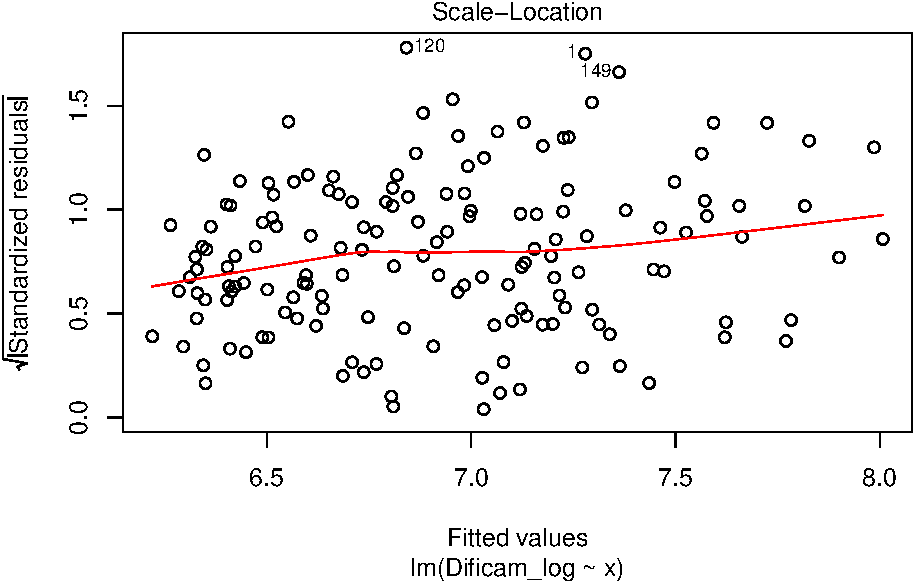
\includegraphics[width=1\linewidth]{img/unnamed-chunk-8-1}

\begin{Shaded}
\begin{Highlighting}[]
\NormalTok{censoT }\OperatorTok\StringTok{ }\KeywordTok{lm}\NormalTok{(Dificam_log}\OperatorTok{~}\StringTok{ }\NormalTok{y, .) }\OperatorTok\StringTok{ }\KeywordTok{plot}\NormalTok{(}\DecValTok{3}\NormalTok{)}
\end{Highlighting}
\end{Shaded}

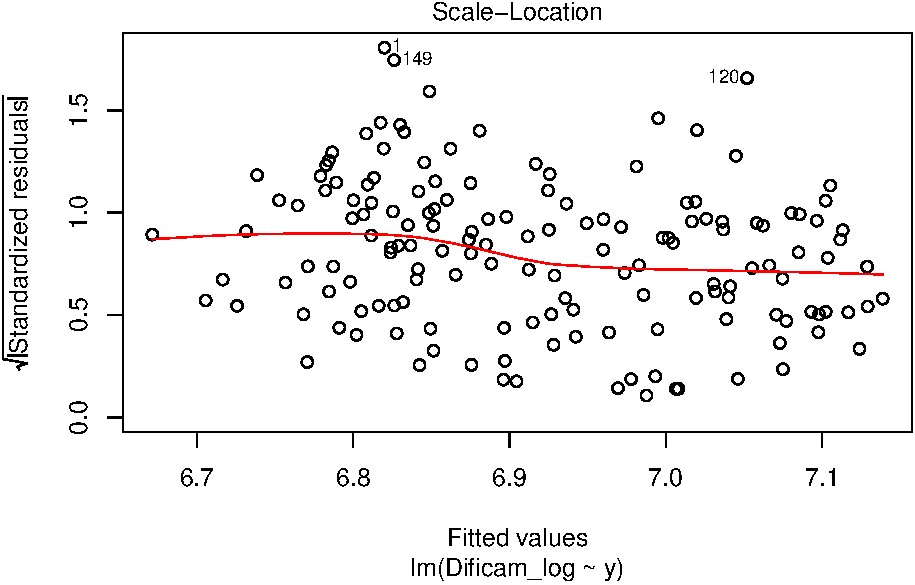
\includegraphics[width=1\linewidth]{img/unnamed-chunk-8-2}

\begin{Shaded}
\begin{Highlighting}[]

\NormalTok{censoT }\OperatorTok\StringTok{ }\KeywordTok{lm}\NormalTok{(Dificam_log}\OperatorTok{~}\StringTok{ }\NormalTok{x, .) }\OperatorTok\StringTok{ }\KeywordTok{bptest}\NormalTok{()  }\CommentTok{#Es mas homocedastica}
\NormalTok{## }
\NormalTok{##  studentized Breusch-Pagan test}
\NormalTok{## }
\NormalTok{## data:  .}
\NormalTok{## BP = 5.6667, df = 1, p-value = 0.01729}
\NormalTok{censoT }\OperatorTok\StringTok{ }\KeywordTok{lm}\NormalTok{(Dificam_log}\OperatorTok{~}\StringTok{ }\NormalTok{y, .) }\OperatorTok\StringTok{ }\KeywordTok{bptest}\NormalTok{()}
\NormalTok{## }
\NormalTok{##  studentized Breusch-Pagan test}
\NormalTok{## }
\NormalTok{## data:  .}
\NormalTok{## BP = 4.6633, df = 1, p-value = 0.03081}
\CommentTok{#El indice de significancia es menor de 0.05, por tanto se rechaza la hipotesis nula}
\end{Highlighting}
\end{Shaded}

\subsection{Test de I de Moran global}\label{test-de-i-de-moran-global}

\begin{Shaded}
\begin{Highlighting}[]
\KeywordTok{moran.test}\NormalTok{(}\DataTypeTok{x=}\NormalTok{Dificam_log, }\DataTypeTok{listw =}\NormalTok{ censo.w.w, }\DataTypeTok{na.action =}\NormalTok{ na.omit)}
\NormalTok{## }
\NormalTok{##  Moran I test under randomisation}
\NormalTok{## }
\NormalTok{## data:  Dificam_log  }
\NormalTok{## weights: censo.w.w    }
\NormalTok{## }
\NormalTok{## Moran I statistic standard deviate = 6.615, p-value = 1.858e-11}
\NormalTok{## alternative hypothesis: greater}
\NormalTok{## sample estimates:}
\NormalTok{## Moran I statistic       Expectation          Variance }
\NormalTok{##       0.333709240      -0.006493506       0.002644972}
\KeywordTok{moran.test}\NormalTok{(}\DataTypeTok{x=}\NormalTok{Dificam_log, }\DataTypeTok{listw =}\NormalTok{ censo.w.b, }\DataTypeTok{na.action =}\NormalTok{ na.omit)  }\CommentTok{#Este nos da el valor mas cercano a 1}
\NormalTok{## }
\NormalTok{##  Moran I test under randomisation}
\NormalTok{## }
\NormalTok{## data:  Dificam_log  }
\NormalTok{## weights: censo.w.b    }
\NormalTok{## }
\NormalTok{## Moran I statistic standard deviate = 8.0524, p-value = 4.061e-16}
\NormalTok{## alternative hypothesis: greater}
\NormalTok{## sample estimates:}
\NormalTok{## Moran I statistic       Expectation          Variance }
\NormalTok{##       0.385389193      -0.006493506       0.002368463}

\CommentTok{# Para los pesos tanto estandarizado como binario, se comprueba que si hay correlación espacial, pues los valores de p fueron menores a 0.05.}
\end{Highlighting}
\end{Shaded}

\subsection{Test de I de Moran Local}\label{test-de-i-de-moran-local}

\begin{Shaded}
\begin{Highlighting}[]
\KeywordTok{moran.plot}\NormalTok{(}\DataTypeTok{x=}\NormalTok{Dificam_log, }\DataTypeTok{listw =}\NormalTok{ censo.w.b)}
\end{Highlighting}
\end{Shaded}

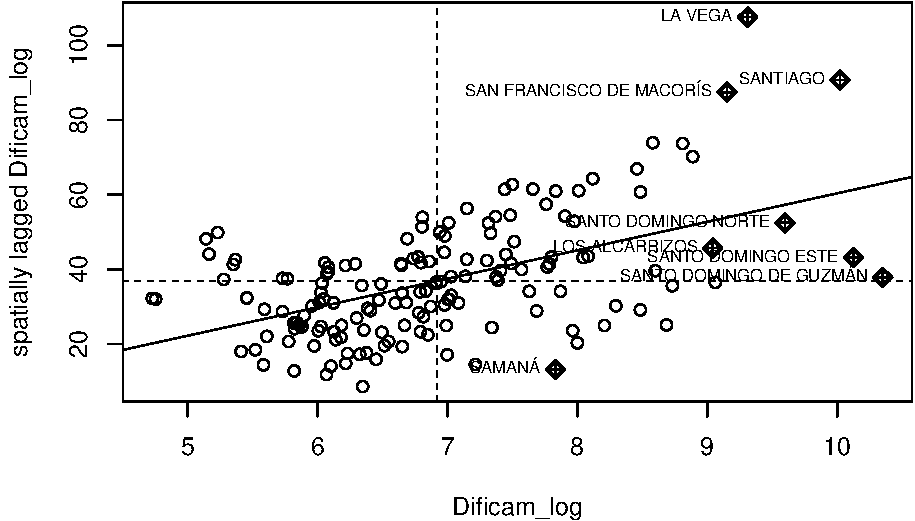
\includegraphics[width=1\linewidth]{img/unnamed-chunk-10-1}

\begin{Shaded}
\begin{Highlighting}[]
\NormalTok{DificamLoc <-}\StringTok{ }\KeywordTok{localmoran}\NormalTok{(Dificam_log, }\DataTypeTok{listw =}\NormalTok{ censo.w.b)}
\KeywordTok{source}\NormalTok{(}\StringTok{'data/lisaclusters.R'}\NormalTok{)}
\KeywordTok{lisamap}\NormalTok{(}\DataTypeTok{objesp =}\NormalTok{ censoT,}
        \DataTypeTok{var =} \StringTok{'Dificam_log'}\NormalTok{,}
        \DataTypeTok{pesos =}\NormalTok{ censo.w.b,}
        \DataTypeTok{tituloleyenda =} \StringTok{'Significancia}\CharTok{\textbackslash{}n}\StringTok{("x-y", léase}\CharTok{\textbackslash{}n}\StringTok{como "x"}\CharTok{\textbackslash{}n}\StringTok{rodeado de "y"'}\NormalTok{, }
        \DataTypeTok{leyenda =}\NormalTok{ T,}
        \DataTypeTok{anchuratitulo =} \DecValTok{1000}\NormalTok{,}
        \DataTypeTok{tamanotitulo =} \DecValTok{16}\NormalTok{,}
        \DataTypeTok{fuentedatos =} \StringTok{'vivpersgeom'}\NormalTok{,}
        \DataTypeTok{titulomapa =} \KeywordTok{paste0}\NormalTok{(}\StringTok{'Clusters LISA de Personas con dificultad para caminar o subir escalones'}\NormalTok{)}
\NormalTok{        )}
\NormalTok{## $grafico}
\end{Highlighting}
\end{Shaded}

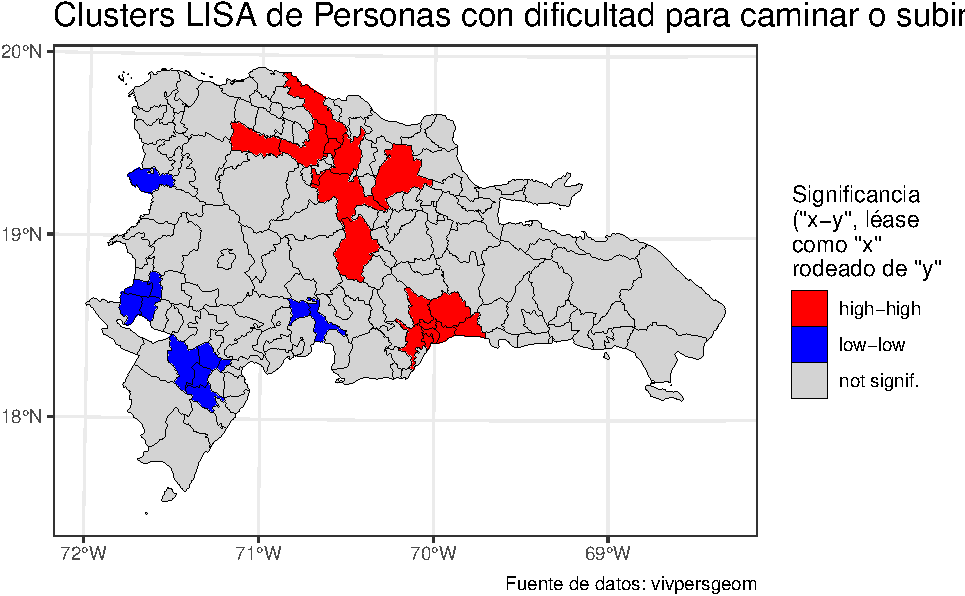
\includegraphics[width=1\linewidth]{img/unnamed-chunk-10-2}

\begin{verbatim}
## 
## $objeto
## Simple feature collection with 155 features and 20 fields
## geometry type:  MULTIPOLYGON
## dimension:      XY
## bbox:           xmin: 182215.8 ymin: 1933532 xmax: 571365.3 ymax: 2205216
## epsg (SRID):    32619
## proj4string:    +proj=utm +zone=19 +datum=WGS84 +units=m +no_defs
## First 10 features:
##                  TOPONIMIA ENLACE
## 1  SANTO DOMINGO DE GUZMÁN 100101
## 2                     AZUA 050201
## 3              LAS CHARCAS 050202
## 4     LAS YAYAS DE VIAJAMA 050203
## 5          PADRE LAS CASAS 050204
## 6                  PERALTA 050205
## 7             SABANA YEGUA 050206
## 8             PUEBLO VIEJO 050207
## 9            TÁBARA ARRIBA 050208
## 10                GUAYABAL 050209
##    Condición de ocupación: Ocupada con personas presentes
## 1                                                  288362
## 2                                                   22797
## 3                                                    3147
## 4                                                    4807
## 5                                                    5243
## 6                                                    3144
## 7                                                    4828
## 8                                                    2689
## 9                                                    4108
## 10                                                   1386
##    Condición de ocupación: Desocupada Población total
## 1                               42200          965040
## 2                                1920           91345
## 3                                 944           11243
## 4                                 798           17620
## 5                                1345           20041
## 6                                 446           15257
## 7                                 594           19020
## 8                                 208           11235
## 9                                 426           17647
## 10                                464            5263
##    Dificultad para Caminar o subir escalones: Si
## 1                                          31271
## 2                                           2616
## 3                                            323
## 4                                            770
## 5                                            804
## 6                                            320
## 7                                            675
## 8                                            266
## 9                                            437
## 10                                           234
##    Asiste o asistió a la escuela: Nunca asistió
## 1                                         45138
## 2                                         12617
## 3                                          2329
## 4                                          3442
## 5                                          4336
## 6                                          3528
## 7                                          2813
## 8                                          1629
## 9                                          3860
## 10                                          909
##    Nivel educativo más alto al que asistió: Preprimaria
## 1                                                 73199
## 2                                                  7718
## 3                                                   965
## 4                                                  1400
## 5                                                  2027
## 6                                                  1360
## 7                                                  1079
## 8                                                   961
## 9                                                  1344
## 10                                                  240
##    Nivel educativo más alto al que asistió: Primaria o básica
## 1                                                      290061
## 2                                                       37701
## 3                                                        5361
## 4                                                        8439
## 5                                                        8458
## 6                                                        5736
## 7                                                        9246
## 8                                                        5270
## 9                                                        7916
## 10                                                       2458
##    Nivel educativo más alto al que asistió: Secundaria o media
## 1                                                       248102
## 2                                                        19003
## 3                                                         1616
## 4                                                         2757
## 5                                                         3104
## 6                                                         2823
## 7                                                         3676
## 8                                                         2133
## 9                                                         2869
## 10                                                         924
##    Nivel educativo más alto al que asistió: Universitaria o superior
## 1                                                             257590
## 2                                                               8601
## 3                                                                204
## 4                                                                541
## 5                                                               1075
## 6                                                               1020
## 7                                                               1048
## 8                                                                484
## 9                                                                602
## 10                                                               479
##    Cantviv PorcPersD PorcPersD_log Dificam_log        x       y
## 1   330562  3.240384     1.1756918   10.350446 400576.8 2044091
## 2    24717  2.863868     1.0521731    7.869402 308829.1 2037708
## 3     4091  2.872899     1.0553215    5.777652 336675.2 2034232
## 4     5605  4.370034     1.4747708    6.646391 289007.6 2058192
## 5     6588  4.011776     1.3892340    6.689599 298570.6 2080773
## 6     3590  2.097398     0.7406975    5.768321 311899.8 2057722
## 7     5422  3.548896     1.2666365    6.514713 300563.9 2037000
## 8     2897  2.367601     0.8618773    5.583496 311931.4 2034599
## 9     4534  2.476342     0.9067823    6.079933 297803.0 2046138
## 10    1850  4.446133     1.4920348    5.455321 313902.6 2070484
##                              geom puntuacionz lagpuntuacionz    quad_sig
## 1  MULTIPOLYGON (((405218.1 20...   3.1437363     9.29680778   high-high
## 2  MULTIPOLYGON (((319065.3 20...   0.8695441    -6.77884923 not signif.
## 3  MULTIPOLYGON (((341415.3 20...  -1.0478095    -0.09622568 not signif.
## 4  MULTIPOLYGON (((304058.1 20...  -0.2515008    -0.38419412 not signif.
## 5  MULTIPOLYGON (((312890.8 20...  -0.2118945    -0.22410831 not signif.
## 6  MULTIPOLYGON (((317370.6 20...  -1.0563629    -3.71835917     low-low
## 7  MULTIPOLYGON (((306745.8 20...  -0.3722002    -1.12696486 not signif.
## 8  MULTIPOLYGON (((310447.9 20...  -1.2257782     0.49734386 not signif.
## 9  MULTIPOLYGON (((306556.7 20...  -0.7707308    -2.10198421 not signif.
## 10 MULTIPOLYGON (((322129.5 20...  -1.3432670    -2.13317172 not signif.
\end{verbatim}

\subsection{Resultado Obtenido}\label{resultado-obtenido}

Se obtuvo un mapa LISA - Local Indicator of Spatial Asociation -, que
nos muestra los clusters de municipios donde existen la mayor y menor
incidencia de casos de personas con dificultad para caminar o subir
escaleras. Encontramos un hotspot en la zona noroeste (municipios en
rojo), donde existe mayor cantidad de personas con dificultad para
caminar o subir escalones; en la región suroeste y fronteriza es donde
existe menos incidencia (municipios en azul); mientras en los demás
municipios (en gris), no se evidencia la incidencia de casos.

\section{FASE 2 - GEOESTADISTICA / ANALISIS
PUNTUAL}\label{fase-2---geoestadistica-analisis-puntual}

\subsection{Metodología}\label{metodologuxeda-1}

Para efectuar este análisis espacial, se cargará la base espacial de
municipios como referencia y el archivo de datos de precipitación de
diferentes años suministrado por la ONAMET. Luego de efectuar el
análisis exploratorio de los datos espaciales (ESDA), obtener las
informaciones estadísticas básicas, histogramas, y efectua pruebas (como
la de Shapiro Wilk) para comprobar que los datos del año seleccionado
tenga una distribución normal, se generan los variogramas modelo, para
seleccionar el idoneo y así efectuar la interpolación (kriging) y
establecer visualmente los municipios con mayor precipitación en el
país.

\subsection{Carga de archivos de datos de precipitaciones. El archivo de
municipios esta ya en
memoria}\label{carga-de-archivos-de-datos-de-precipitaciones.-el-archivo-de-municipios-esta-ya-en-memoria}

\begin{Shaded}
\begin{Highlighting}[]
\NormalTok{prec <-}\StringTok{ }\KeywordTok{st_read}\NormalTok{(}\StringTok{'data/onamet_prec_anual_sf.gpkg'}\NormalTok{)}
\NormalTok{## Reading layer `onamet_prec_anual_sf' from data source `/home/lbine/unidad-0-asignacion-99-mi-proyecto-wlbinet1/data/onamet_prec_anual_sf.gpkg' using driver `GPKG'}
\NormalTok{## Simple feature collection with 25 features and 37 fields}
\NormalTok{## geometry type:  POINT}
\NormalTok{## dimension:      XY}
\NormalTok{## bbox:           xmin: -71.7 ymin: 18.067 xmax: -68.367 ymax: 19.85}
\NormalTok{## epsg (SRID):    4326}
\NormalTok{## proj4string:    +proj=longlat +datum=WGS84 +no_defs}
\KeywordTok{st_crs}\NormalTok{(prec)}
\NormalTok{## Coordinate Reference System:}
\NormalTok{##   EPSG: 4326 }
\NormalTok{##   proj4string: "+proj=longlat +datum=WGS84 +no_defs"}
\NormalTok{crswgs84utm <-}\StringTok{ }\DecValTok{32619}
\NormalTok{precUtm <-}\StringTok{ }\NormalTok{prec }\OperatorTok\StringTok{ }\KeywordTok{st_transform}\NormalTok{(}\DataTypeTok{crs =}\NormalTok{ crswgs84utm)}
\end{Highlighting}
\end{Shaded}

\subsection{ESDA}\label{esda}

\begin{Shaded}
\begin{Highlighting}[]
\KeywordTok{nrow}\NormalTok{(precUtm)}
\NormalTok{## [1] 25}
\NormalTok{prec82 <-}\StringTok{ }\NormalTok{precUtm}\OperatorTok{$}\StringTok{`}\DataTypeTok{a1982}\StringTok{`}   \CommentTok{# Seleccion de variable}

\KeywordTok{hist}\NormalTok{(prec82)}
\end{Highlighting}
\end{Shaded}

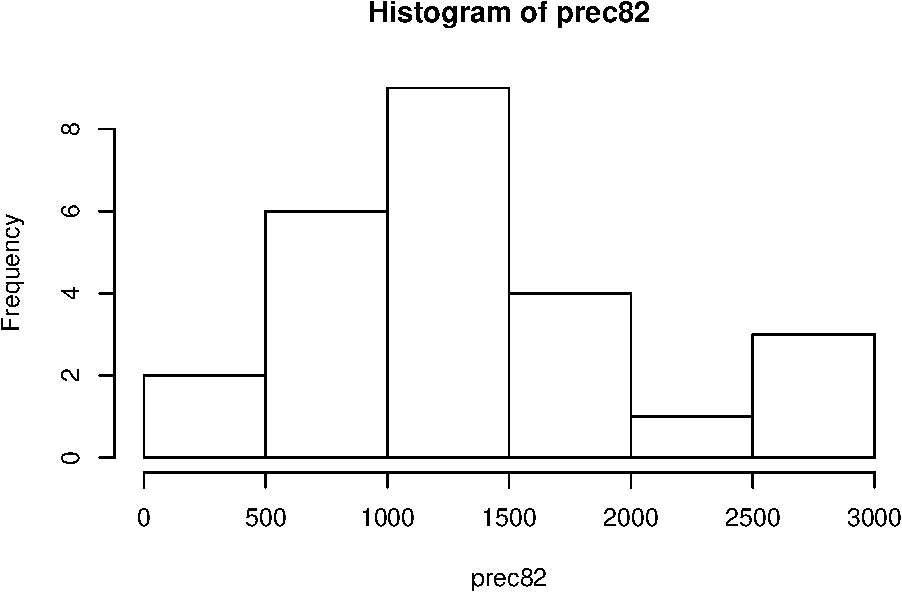
\includegraphics[width=1\linewidth]{img/unnamed-chunk-12-1}

\begin{Shaded}
\begin{Highlighting}[]
\KeywordTok{hist}\NormalTok{(}\KeywordTok{log}\NormalTok{(prec82))}
\end{Highlighting}
\end{Shaded}

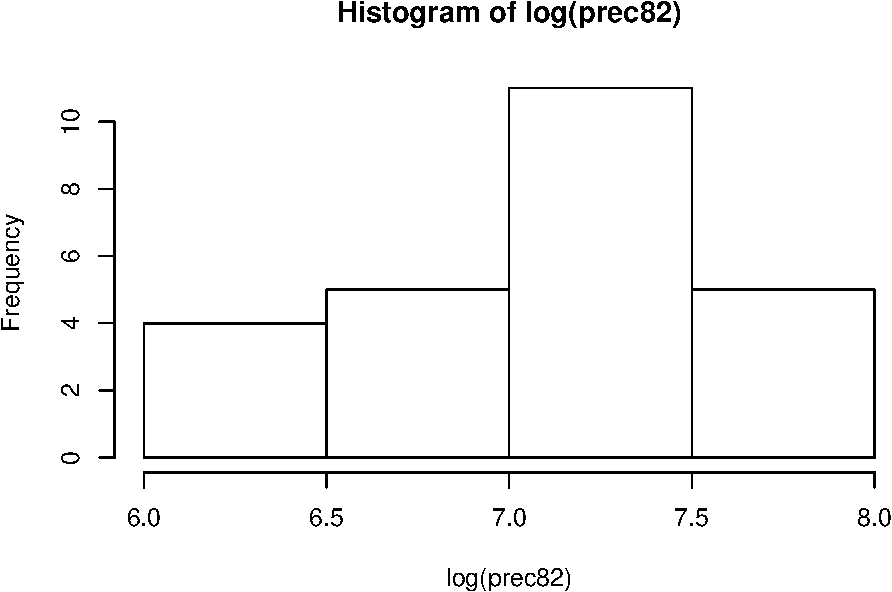
\includegraphics[width=1\linewidth]{img/unnamed-chunk-12-2}

\begin{Shaded}
\begin{Highlighting}[]
\KeywordTok{shapiro.test}\NormalTok{(prec82)}
\NormalTok{## }
\NormalTok{##  Shapiro-Wilk normality test}
\NormalTok{## }
\NormalTok{## data:  prec82}
\NormalTok{## W = 0.94689, p-value = 0.2131}
\KeywordTok{shapiro.test}\NormalTok{(}\KeywordTok{log}\NormalTok{(prec82))}
\NormalTok{## }
\NormalTok{##  Shapiro-Wilk normality test}
\NormalTok{## }
\NormalTok{## data:  log(prec82)}
\NormalTok{## W = 0.94321, p-value = 0.1755}
\KeywordTok{qqnorm}\NormalTok{(prec82)}
\end{Highlighting}
\end{Shaded}

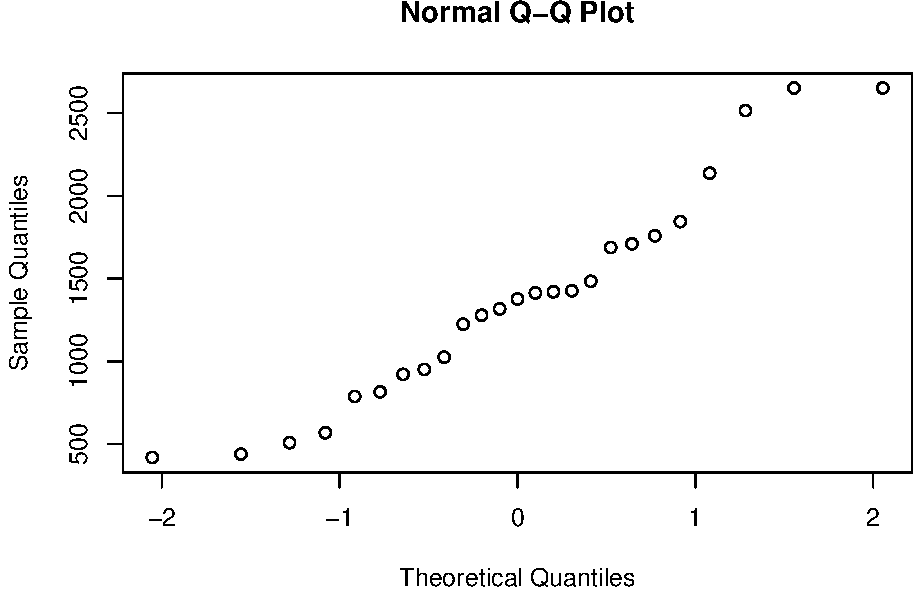
\includegraphics[width=1\linewidth]{img/unnamed-chunk-12-3}

\begin{Shaded}
\begin{Highlighting}[]
\KeywordTok{qqnorm}\NormalTok{(}\KeywordTok{log}\NormalTok{(prec82))}
\end{Highlighting}
\end{Shaded}

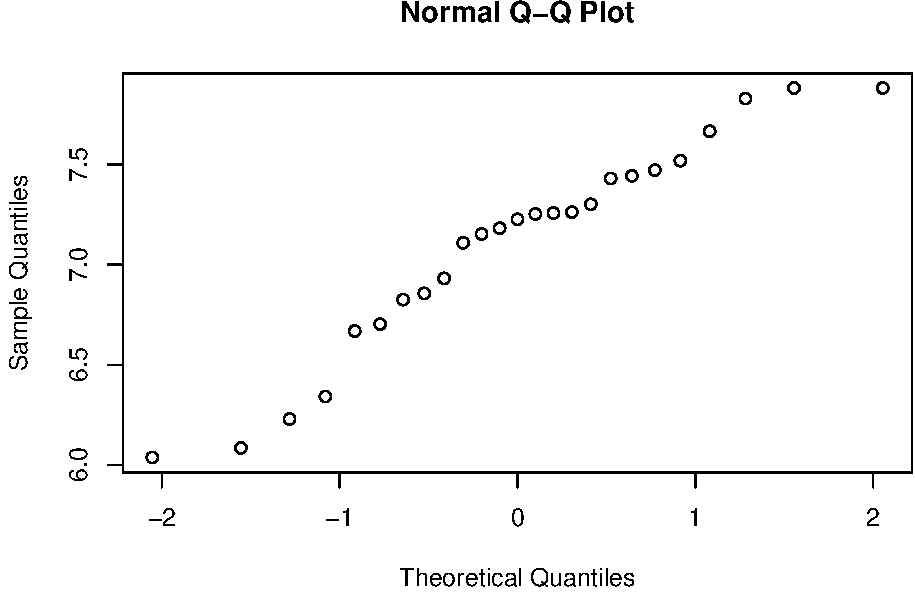
\includegraphics[width=1\linewidth]{img/unnamed-chunk-12-4}

\begin{Shaded}
\begin{Highlighting}[]

\NormalTok{preci <-}\StringTok{ }\KeywordTok{na.omit}\NormalTok{(precUtm[,}\KeywordTok{c}\NormalTok{(}\StringTok{'Estación', '}\NormalTok{a1982}\StringTok{')])}
\StringTok{preci$a1982log <- log(preci$a1982)}
\StringTok{preci}
\StringTok{## Simple feature collection with 25 features and 3 fields}
\StringTok{## geometry type:  POINT}
\StringTok{## dimension:      XY}
\StringTok{## bbox:           xmin: 215264.1 ymin: 1999092 xmax: 566794.7 ymax: 2197035}
\StringTok{## epsg (SRID):    32619}
\StringTok{## proj4string:    +proj=utm +zone=19 +datum=WGS84 +units=m +no_defs}
\StringTok{## First 10 features:}
\StringTok{##            Estación  a1982                     geom a1982log}
\StringTok{## 1          Barahona  815.3 POINT (277900.2 2013585) 6.703556}
\StringTok{## 2         Bayaguana 1758.6 POINT (433242.1 2073284) 7.472273}
\StringTok{## 3           Cabrera 2136.9   POINT (405636 2171119) 7.667111}
\StringTok{## 4         Constanza  921.2 POINT (320947.7 2090623) 6.825677}
\StringTok{## 5  Gaspar Hernández 1844.1 POINT (363678.2 2169619) 7.519747}
\StringTok{## 6       Hondo Valle 1709.9 POINT (215264.1 2071669) 7.444190}
\StringTok{## 7            Jimaní  507.5 POINT (221953.7 2045651) 6.229497}
\StringTok{## 8          La Unión 1413.1 POINT (337592.1 2184559) 7.253541}
\StringTok{## 9           La Vega 1483.2 POINT (338847.1 2125548) 7.301957}
\StringTok{## 10     Las Américas  787.4 POINT (429562.7 2038222) 6.668736}
\end{Highlighting}
\end{Shaded}

\subsection{Despliega la localizacion de los
observatorios}\label{despliega-la-localizacion-de-los-observatorios}

\begin{Shaded}
\begin{Highlighting}[]
\KeywordTok{library}\NormalTok{(ggplot2)}

\KeywordTok{ggplot}\NormalTok{() }\OperatorTok{+}
\StringTok{  }\KeywordTok{geom_sf}\NormalTok{(}\DataTypeTok{data =}\NormalTok{ muni.sf, }\DataTypeTok{fill =} \StringTok{'white'}\NormalTok{) }\OperatorTok{+}
\StringTok{  }\KeywordTok{geom_sf}\NormalTok{(}\DataTypeTok{data =}\NormalTok{ preci, }\KeywordTok{aes}\NormalTok{(}\DataTypeTok{col =}\NormalTok{ a1982log), }\DataTypeTok{size =} \DecValTok{6}\NormalTok{) }\OperatorTok{+}
\StringTok{  }\KeywordTok{scale_colour_gradient}\NormalTok{(}\DataTypeTok{low=}\StringTok{"#deebf7"}\NormalTok{, }\DataTypeTok{high=}\StringTok{"#3182bd"}\NormalTok{) }\OperatorTok{+}
\StringTok{  }\KeywordTok{geom_sf_text}\NormalTok{(}\DataTypeTok{data =}\NormalTok{ muni.sf, }\KeywordTok{aes}\NormalTok{(}\DataTypeTok{label=}\NormalTok{TOPONIMIA), }\DataTypeTok{check_overlap =}\NormalTok{ T, }\DataTypeTok{size =} \DecValTok{2}\NormalTok{) }\OperatorTok{+}
\StringTok{  }\KeywordTok{geom_sf_text}\NormalTok{(}\DataTypeTok{data =}\NormalTok{ preci, }\KeywordTok{aes}\NormalTok{(}\DataTypeTok{label=}\NormalTok{Estación), }\DataTypeTok{check_overlap =}\NormalTok{ T, }\DataTypeTok{size =} \FloatTok{1.5}\NormalTok{) }\OperatorTok{+}
\StringTok{  }\KeywordTok{theme_bw}\NormalTok{()}
\end{Highlighting}
\end{Shaded}

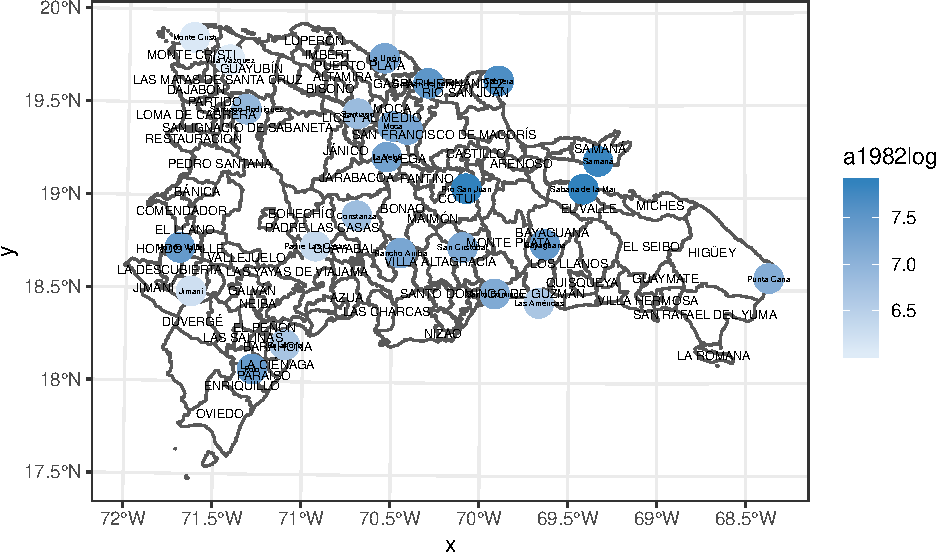
\includegraphics[width=1\linewidth]{img/unnamed-chunk-13-1}

\subsection{variograma muestral}\label{variograma-muestral}

\begin{Shaded}
\begin{Highlighting}[]
\NormalTok{v82 <-}\StringTok{ }\KeywordTok{variogram}\NormalTok{(a1982log}\OperatorTok{~}\DecValTok{1}\NormalTok{, preci)}
\NormalTok{v82}
\NormalTok{##    np       dist        gamma dir.hor dir.ver   id}
\NormalTok{## 1   1   8896.559 1.075597e-05       0       0 var1}
\NormalTok{## 2   7  22355.182 1.555620e-01       0       0 var1}
\NormalTok{## 3  12  31950.749 1.304567e-01       0       0 var1}
\NormalTok{## 4   8  40371.385 4.236860e-02       0       0 var1}
\NormalTok{## 5   7  50078.452 1.999113e-01       0       0 var1}
\NormalTok{## 6  14  58855.498 1.253300e-01       0       0 var1}
\NormalTok{## 7  12  67482.051 1.439899e-01       0       0 var1}
\NormalTok{## 8   9  77223.824 1.703296e-01       0       0 var1}
\NormalTok{## 9  23  85146.530 2.234314e-01       0       0 var1}
\NormalTok{## 10 12  93304.363 3.132216e-01       0       0 var1}
\NormalTok{## 11 11 103535.175 1.628902e-01       0       0 var1}
\NormalTok{## 12 19 112257.676 2.782182e-01       0       0 var1}
\NormalTok{## 13 18 120004.515 2.351375e-01       0       0 var1}
\NormalTok{## 14 14 128628.216 2.520859e-01       0       0 var1}
\KeywordTok{plot}\NormalTok{(v82, }\DataTypeTok{plot.numbers =}\NormalTok{ T)}
\end{Highlighting}
\end{Shaded}

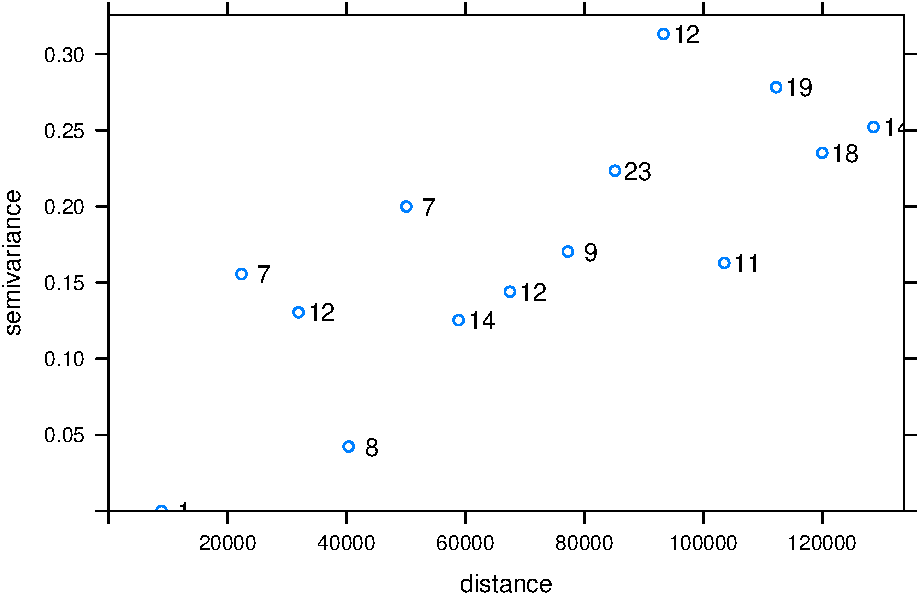
\includegraphics[width=1\linewidth]{img/unnamed-chunk-14-1}

\subsection{variograma modelo}\label{variograma-modelo}

\begin{Shaded}
\begin{Highlighting}[]
\NormalTok{v82_m <-}\StringTok{ }\KeywordTok{fit.variogram}\NormalTok{(v82, }\KeywordTok{vgm}\NormalTok{(}\DataTypeTok{model =} \StringTok{"Sph"}\NormalTok{, }\DataTypeTok{range =} \DecValTok{50000}\NormalTok{))}
\NormalTok{v82_m}
\NormalTok{##   model     psill    range}
\NormalTok{## 1   Sph 0.2290492 96599.97}
\KeywordTok{plot}\NormalTok{(v82, v82_m, }\DataTypeTok{plot.numbers =}\NormalTok{ T)}
\end{Highlighting}
\end{Shaded}

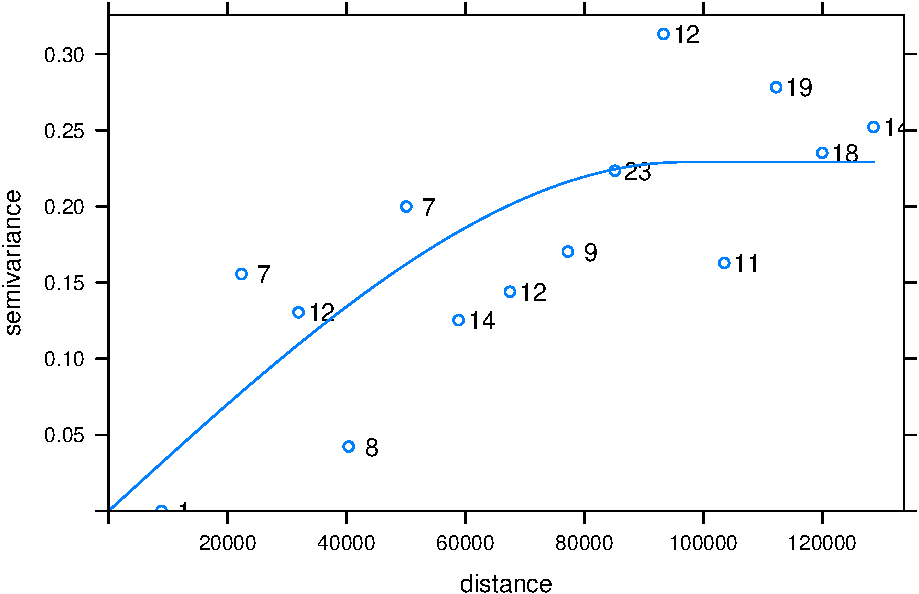
\includegraphics[width=1\linewidth]{img/unnamed-chunk-15-1}

\begin{Shaded}
\begin{Highlighting}[]

\NormalTok{v82_m2 <-}\StringTok{ }\KeywordTok{fit.variogram}\NormalTok{(v82, }\KeywordTok{vgm}\NormalTok{(}\DataTypeTok{model =} \StringTok{"Exp"}\NormalTok{, }\DataTypeTok{range =} \DecValTok{50000}\NormalTok{))}
\NormalTok{v82_m2}
\NormalTok{##   model     psill    range}
\NormalTok{## 1   Exp 0.2507095 48191.96}
\KeywordTok{plot}\NormalTok{(v82, v82_m2, }\DataTypeTok{plot.numbers =}\NormalTok{ T)}
\end{Highlighting}
\end{Shaded}

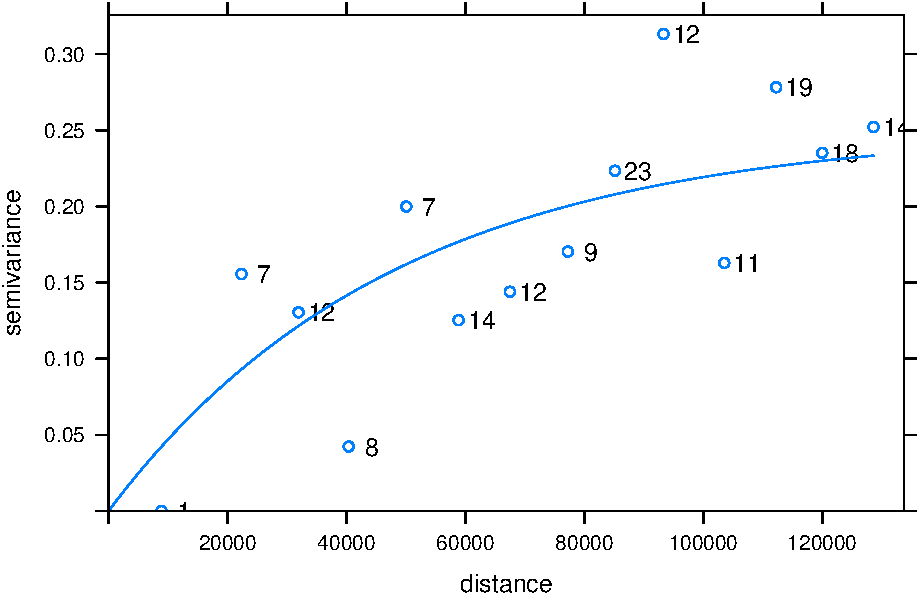
\includegraphics[width=1\linewidth]{img/unnamed-chunk-15-2}

\begin{Shaded}
\begin{Highlighting}[]

\NormalTok{v82_m3 <-}\StringTok{ }\KeywordTok{fit.variogram}\NormalTok{(v82, }\KeywordTok{vgm}\NormalTok{(}\DataTypeTok{model =} \StringTok{"Gau"}\NormalTok{, }\DataTypeTok{range =} \DecValTok{50000}\NormalTok{))}
\NormalTok{v82_m3}
\NormalTok{##   model     psill    range}
\NormalTok{## 1   Gau 0.1701203 21015.34}
\KeywordTok{plot}\NormalTok{(v82, v82_m3, }\DataTypeTok{plot.numbers =}\NormalTok{ T)}
\end{Highlighting}
\end{Shaded}

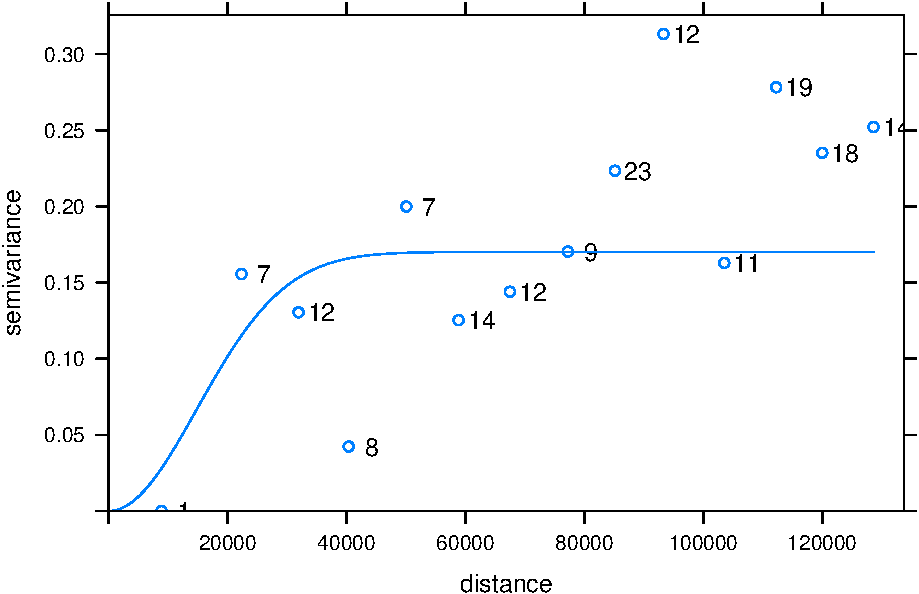
\includegraphics[width=1\linewidth]{img/unnamed-chunk-15-3}

\begin{Shaded}
\begin{Highlighting}[]

\KeywordTok{attr}\NormalTok{(v82_m, }\StringTok{'SSErr'}\NormalTok{)}
\NormalTok{## [1] 1.919642e-10}
\KeywordTok{attr}\NormalTok{(v82_m2, }\StringTok{'SSErr'}\NormalTok{)               }\CommentTok{#Elegimos el modelo exponencial}
\NormalTok{## [1] 1.706493e-10}
\KeywordTok{attr}\NormalTok{(v82_m3, }\StringTok{'SSErr'}\NormalTok{)}
\NormalTok{## [1] 1.919187e-10}
\end{Highlighting}
\end{Shaded}

\subsection{kriging ordinario}\label{kriging-ordinario}

\begin{Shaded}
\begin{Highlighting}[]
\CommentTok{# creacion de cuadricula de 1000}
\NormalTok{grd <-}\StringTok{ }\KeywordTok{st_bbox}\NormalTok{(muni.sf) }\OperatorTok
\StringTok{  }\KeywordTok{st_as_stars}\NormalTok{(}\DataTypeTok{dx =} \DecValTok{1000}\NormalTok{) }\OperatorTok\StringTok{ }\CommentTok{#10000 metros=10km de resolución espacial}
\StringTok{  }\KeywordTok{st_set_crs}\NormalTok{(crswgs84utm ) }\OperatorTok
\StringTok{  }\KeywordTok{st_crop}\NormalTok{(muni.sf)}
\NormalTok{grd}
\NormalTok{## stars object with 2 dimensions and 1 attribute}
\NormalTok{## attribute(s):}
\NormalTok{##     values      }
\NormalTok{##  Min.   :0      }
\NormalTok{##  1st Qu.:0      }
\NormalTok{##  Median :0      }
\NormalTok{##  Mean   :0      }
\NormalTok{##  3rd Qu.:0      }
\NormalTok{##  Max.   :0      }
\NormalTok{##  NA's   :58018  }
\NormalTok{## dimension(s):}
\NormalTok{##   from  to  offset delta                       refsys point values    }
\NormalTok{## x    1 390  182216  1000 +proj=utm +zone=19 +datum...    NA   NULL [x]}
\NormalTok{## y    1 272 2205216 -1000 +proj=utm +zone=19 +datum...    NA   NULL [y]}
\KeywordTok{plot}\NormalTok{(grd)}
\end{Highlighting}
\end{Shaded}

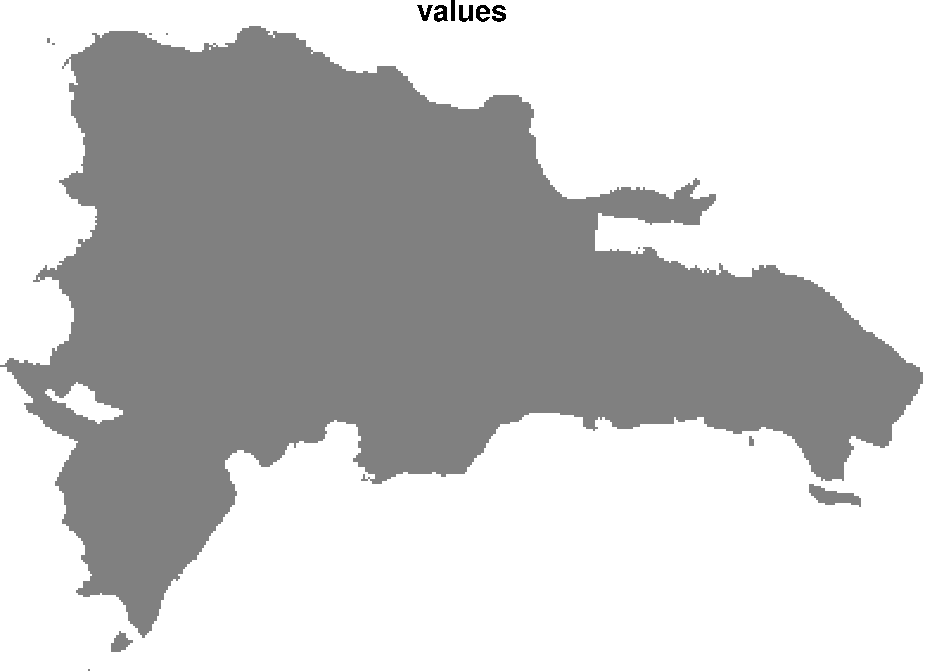
\includegraphics[width=1\linewidth]{img/unnamed-chunk-16-1}

\begin{Shaded}
\begin{Highlighting}[]

\CommentTok{# interpolacion}
\NormalTok{k <-}\StringTok{ }\KeywordTok{krige}\NormalTok{(}\DataTypeTok{formula =}\NormalTok{ a1982log}\OperatorTok{~}\DecValTok{1}\NormalTok{, }\DataTypeTok{locations =}\NormalTok{ preci, }\DataTypeTok{newdata =}\NormalTok{ grd, }\DataTypeTok{model =}\NormalTok{ v82_m2)}
\NormalTok{## [using ordinary kriging]}
\NormalTok{k}
\NormalTok{## stars object with 2 dimensions and 2 attributes}
\NormalTok{## attribute(s):}
\NormalTok{##    var1.pred       var1.var     }
\NormalTok{##  Min.   :6.05    Min.   :0.00   }
\NormalTok{##  1st Qu.:6.83    1st Qu.:0.09   }
\NormalTok{##  Median :7.08    Median :0.13   }
\NormalTok{##  Mean   :7.07    Mean   :0.13   }
\NormalTok{##  3rd Qu.:7.28    3rd Qu.:0.16   }
\NormalTok{##  Max.   :7.88    Max.   :0.26   }
\NormalTok{##  NA's   :58018   NA's   :58018  }
\NormalTok{## dimension(s):}
\NormalTok{##   from  to  offset delta                       refsys point values    }
\NormalTok{## x    1 390  182216  1000 +proj=utm +zone=19 +datum...    NA   NULL [x]}
\NormalTok{## y    1 272 2205216 -1000 +proj=utm +zone=19 +datum...    NA   NULL [y]}
\KeywordTok{plot}\NormalTok{(k)}
\end{Highlighting}
\end{Shaded}

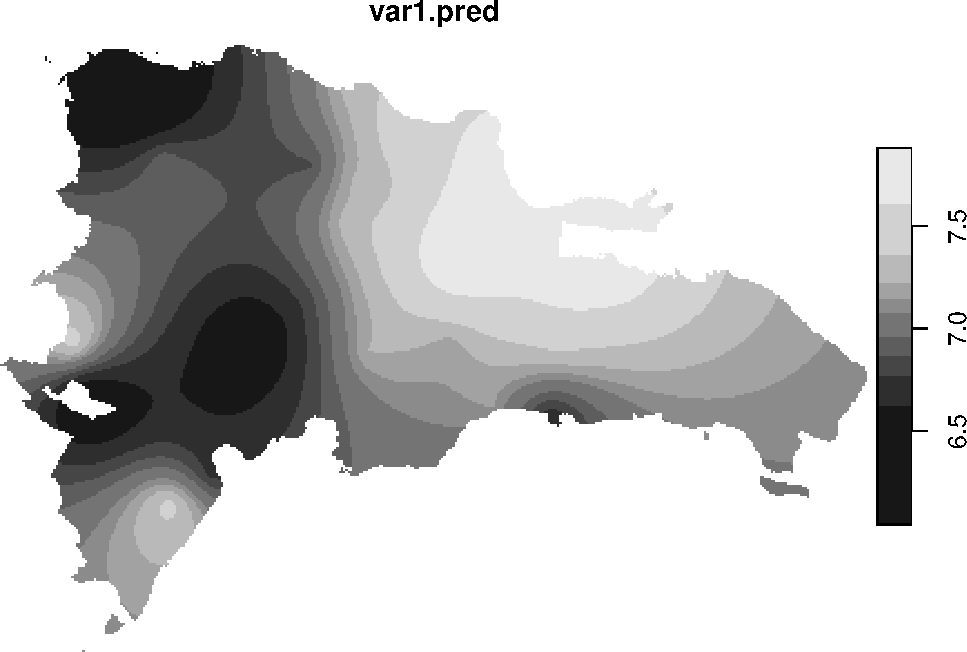
\includegraphics[width=1\linewidth]{img/unnamed-chunk-16-2}

\begin{Shaded}
\begin{Highlighting}[]
\KeywordTok{ggplot}\NormalTok{() }\OperatorTok{+}
\StringTok{  }\KeywordTok{geom_stars}\NormalTok{(}\DataTypeTok{data =}\NormalTok{ k, }\KeywordTok{aes}\NormalTok{(}\DataTypeTok{fill =}\NormalTok{ var1.pred, }\DataTypeTok{x =}\NormalTok{ x, }\DataTypeTok{y =}\NormalTok{ y)) }\OperatorTok{+}\StringTok{ }
\StringTok{  }\KeywordTok{scale_fill_gradient}\NormalTok{(}\DataTypeTok{low=}\StringTok{"#deebf7"}\NormalTok{, }\DataTypeTok{high=}\StringTok{"#3182bd"}\NormalTok{) }\OperatorTok{+}
\StringTok{  }\KeywordTok{geom_sf}\NormalTok{(}\DataTypeTok{data =} \KeywordTok{st_cast}\NormalTok{(muni.sf, }\StringTok{"MULTILINESTRING"}\NormalTok{)) }\OperatorTok{+}
\StringTok{  }\KeywordTok{geom_sf}\NormalTok{(}\DataTypeTok{data =}\NormalTok{ preci) }\OperatorTok{+}
\StringTok{  }\KeywordTok{geom_sf_text}\NormalTok{(}\DataTypeTok{data =}\NormalTok{ muni.sf, }\KeywordTok{aes}\NormalTok{(}\DataTypeTok{label=}\NormalTok{TOPONIMIA), }\DataTypeTok{check_overlap =}\NormalTok{ T, }\DataTypeTok{size =} \DecValTok{2}\NormalTok{) }\OperatorTok{+}
\StringTok{  }\KeywordTok{theme_bw}\NormalTok{()}
\end{Highlighting}
\end{Shaded}

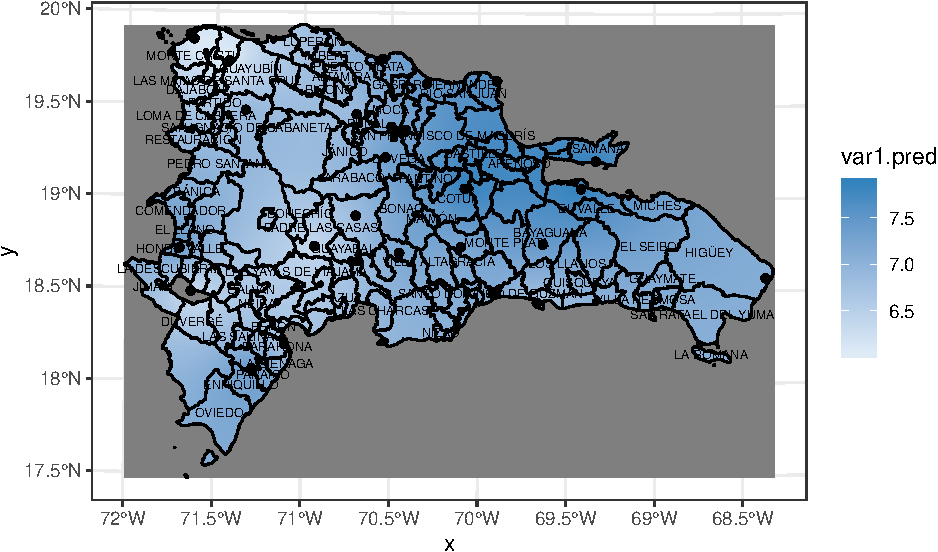
\includegraphics[width=1\linewidth]{img/unnamed-chunk-17-1}

\subsection{Para conseguir los valores reales de las
precipitaciones}\label{para-conseguir-los-valores-reales-de-las-precipitaciones}

\begin{Shaded}
\begin{Highlighting}[]
\KeywordTok{ggplot}\NormalTok{() }\OperatorTok{+}
\StringTok{  }\KeywordTok{geom_stars}\NormalTok{(}\DataTypeTok{data =} \KeywordTok{exp}\NormalTok{(k), }\KeywordTok{aes}\NormalTok{(}\DataTypeTok{fill =}\NormalTok{ var1.pred, }\DataTypeTok{x =}\NormalTok{ x, }\DataTypeTok{y =}\NormalTok{ y)) }\OperatorTok{+}\StringTok{ }
\StringTok{  }\KeywordTok{scale_fill_gradient}\NormalTok{(}\DataTypeTok{low=}\StringTok{"#deebf7"}\NormalTok{, }\DataTypeTok{high=}\StringTok{"#3182bd"}\NormalTok{, }\DataTypeTok{trans =} \StringTok{'log10'}\NormalTok{) }\OperatorTok{+}
\StringTok{  }\KeywordTok{geom_sf}\NormalTok{(}\DataTypeTok{data =} \KeywordTok{st_cast}\NormalTok{(muni.sf, }\StringTok{"MULTILINESTRING"}\NormalTok{)) }\OperatorTok{+}
\StringTok{  }\KeywordTok{geom_sf}\NormalTok{(}\DataTypeTok{data =}\NormalTok{ preci) }\OperatorTok{+}
\StringTok{  }\KeywordTok{geom_sf_text}\NormalTok{(}\DataTypeTok{data =}\NormalTok{ muni.sf, }\KeywordTok{aes}\NormalTok{(}\DataTypeTok{label=}\NormalTok{TOPONIMIA), }\DataTypeTok{check_overlap =}\NormalTok{ T, }\DataTypeTok{size =} \DecValTok{2}\NormalTok{) }\OperatorTok{+}
\StringTok{  }\KeywordTok{theme_bw}\NormalTok{()}
\end{Highlighting}
\end{Shaded}

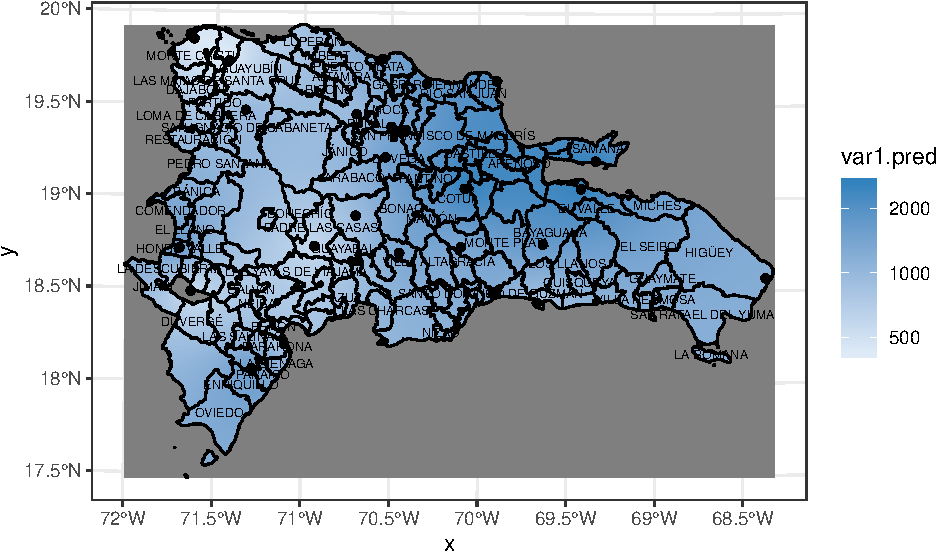
\includegraphics[width=1\linewidth]{img/unnamed-chunk-18-1}

\subsection{Resultado obtenido del Análisis de
precipitaciones}\label{resultado-obtenido-del-anuxe1lisis-de-precipitaciones}

El analisis Kriging ordinario evidencia de una manera muy puntual aunque
segregada, que los municipios localizados en la region nordeste del
país, recibieron una mayor cantidad de precipitaciones para el periodo
correspondiente al año 1982.

\section{FASE 3 - MODELIZACIÓN}\label{fase-3---modelizaciuxf3n}

\subsection{Metodología}\label{metodologuxeda-2}

Acá se determinará la relación existente entre la variable que señala a
las personas que tienen dificultad para caminar o subir escalones en el
pais y las de nivel educativo más alto al que asistió. Para esto se
cargan las variables a relacionar de la base de datos del censo. Se
calculan los valores porcentuales con respecto a la población total del
país para 2010 y su valores logaritmicos. Y a partir de estos valores,
se construye el modelo lineal y el modelo espacial autorregresivo.

\subsection{Cargado de los datos}\label{cargado-de-los-datos}

\begin{Shaded}
\begin{Highlighting}[]
\NormalTok{varsel <-}\StringTok{ }\NormalTok{censoT }\OperatorTok\StringTok{ }\NormalTok{dplyr}\OperatorTok{::}\KeywordTok{select}\NormalTok{(}
  \DataTypeTok{Toponimia =}\NormalTok{ TOPONIMIA,}
  \DataTypeTok{PoblTotal =} \StringTok{"Población total"}\NormalTok{,}
  \DataTypeTok{PersDif =} \StringTok{"Dificultad para Caminar o subir escalones: Si"}\NormalTok{,}
  \DataTypeTok{Noasistio =}  \StringTok{"Asiste o asistió a la escuela: Nunca asistió",}
\StringTok{  Preprimaria = "}\NormalTok{Nivel educativo más alto al que asistió: Preprimaria}\StringTok{",}
\StringTok{  Primaria = "}\NormalTok{Nivel educativo más alto al que asistió: Primaria o básica}\StringTok{",}
\StringTok{  Secundaria = "}\NormalTok{Nivel educativo más alto al que asistió: Secundaria o media}\StringTok{",}
\StringTok{  Universidad = "}\NormalTok{Nivel educativo más alto al que asistió: Universitaria o superior}\StringTok{")}
\StringTok{varsel}
\StringTok{## Simple feature collection with 155 features and 8 fields}
\StringTok{## geometry type:  MULTIPOLYGON}
\StringTok{## dimension:      XY}
\StringTok{## bbox:           xmin: 182215.8 ymin: 1933532 xmax: 571365.3 ymax: 2205216}
\StringTok{## epsg (SRID):    32619}
\StringTok{## proj4string:    +proj=utm +zone=19 +datum=WGS84 +units=m +no_defs}
\StringTok{## First 10 features:}
\StringTok{##                  Toponimia PoblTotal PersDif Noasistio Preprimaria}
\StringTok{## 1  SANTO DOMINGO DE GUZMÁN    965040   31271     45138       73199}
\StringTok{## 2                     AZUA     91345    2616     12617        7718}
\StringTok{## 3              LAS CHARCAS     11243     323      2329         965}
\StringTok{## 4     LAS YAYAS DE VIAJAMA     17620     770      3442        1400}
\StringTok{## 5          PADRE LAS CASAS     20041     804      4336        2027}
\StringTok{## 6                  PERALTA     15257     320      3528        1360}
\StringTok{## 7             SABANA YEGUA     19020     675      2813        1079}
\StringTok{## 8             PUEBLO VIEJO     11235     266      1629         961}
\StringTok{## 9            TÁBARA ARRIBA     17647     437      3860        1344}
\StringTok{## 10                GUAYABAL      5263     234       909         240}
\StringTok{##    Primaria Secundaria Universidad                           geom}
\StringTok{## 1    290061     248102      257590 MULTIPOLYGON (((405218.1 20...}
\StringTok{## 2     37701      19003        8601 MULTIPOLYGON (((319065.3 20...}
\StringTok{## 3      5361       1616         204 MULTIPOLYGON (((341415.3 20...}
\StringTok{## 4      8439       2757         541 MULTIPOLYGON (((304058.1 20...}
\StringTok{## 5      8458       3104        1075 MULTIPOLYGON (((312890.8 20...}
\StringTok{## 6      5736       2823        1020 MULTIPOLYGON (((317370.6 20...}
\StringTok{## 7      9246       3676        1048 MULTIPOLYGON (((306745.8 20...}
\StringTok{## 8      5270       2133         484 MULTIPOLYGON (((310447.9 20...}
\StringTok{## 9      7916       2869         602 MULTIPOLYGON (((306556.7 20...}
\StringTok{## 10     2458        924         479 MULTIPOLYGON (((322129.5 20...}
\end{Highlighting}
\end{Shaded}

\subsection{Relativización de los datos con el campo del total de
Población. Se genera las columnas de porcentaje de los datos y al mismo
tiempo los logaritmos de los porcentajes
encontrados.}\label{relativizaciuxf3n-de-los-datos-con-el-campo-del-total-de-poblaciuxf3n.-se-genera-las-columnas-de-porcentaje-de-los-datos-y-al-mismo-tiempo-los-logaritmos-de-los-porcentajes-encontrados.}

\begin{Shaded}
\begin{Highlighting}[]
\NormalTok{varsellog <-}\StringTok{ }\NormalTok{varsel }\OperatorTok\StringTok{ }\KeywordTok{mutate_each}\NormalTok{(}
  \KeywordTok{funs}\NormalTok{(}\DataTypeTok{PCT=}\KeywordTok{round}\NormalTok{(.}\OperatorTok{/}\NormalTok{PoblTotal,}\DecValTok{4}\NormalTok{)}\OperatorTok{*}\DecValTok{100}\NormalTok{,}
       \DataTypeTok{PCTLOG=}\KeywordTok{log1p}\NormalTok{(}\KeywordTok{round}\NormalTok{(.}\OperatorTok{/}\NormalTok{PoblTotal,}\DecValTok{4}\NormalTok{)}\OperatorTok{*}\DecValTok{100}\NormalTok{)),}
  \OperatorTok{-}\DecValTok{1}\NormalTok{, }\OperatorTok{-}\DecValTok{2}\NormalTok{, }\OperatorTok{-}\NormalTok{geom, }\OperatorTok{-}\NormalTok{PoblTotal)}
\NormalTok{## Warning: funs() is soft deprecated as of dplyr 0.8.0}
\NormalTok{## Please use a list of either functions or lambdas: }
\NormalTok{## }
\NormalTok{##   # Simple named list: }
\NormalTok{##   list(mean = mean, median = median)}
\NormalTok{## }
\NormalTok{##   # Auto named with `tibble::lst()`: }
\NormalTok{##   tibble::lst(mean, median)}
\NormalTok{## }
\NormalTok{##   # Using lambdas}
\NormalTok{##   list(~ mean(., trim = .2), ~ median(., na.rm = TRUE))}
\NormalTok{## This warning is displayed once per session.}
\NormalTok{varsellog}
\NormalTok{## Simple feature collection with 155 features and 20 fields}
\NormalTok{## geometry type:  MULTIPOLYGON}
\NormalTok{## dimension:      XY}
\NormalTok{## bbox:           xmin: 182215.8 ymin: 1933532 xmax: 571365.3 ymax: 2205216}
\NormalTok{## epsg (SRID):    32619}
\NormalTok{## proj4string:    +proj=utm +zone=19 +datum=WGS84 +units=m +no_defs}
\NormalTok{## First 10 features:}
\NormalTok{##                  Toponimia PoblTotal PersDif Noasistio Preprimaria}
\NormalTok{## 1  SANTO DOMINGO DE GUZMÁN    965040   31271     45138       73199}
\NormalTok{## 2                     AZUA     91345    2616     12617        7718}
\NormalTok{## 3              LAS CHARCAS     11243     323      2329         965}
\NormalTok{## 4     LAS YAYAS DE VIAJAMA     17620     770      3442        1400}
\NormalTok{## 5          PADRE LAS CASAS     20041     804      4336        2027}
\NormalTok{## 6                  PERALTA     15257     320      3528        1360}
\NormalTok{## 7             SABANA YEGUA     19020     675      2813        1079}
\NormalTok{## 8             PUEBLO VIEJO     11235     266      1629         961}
\NormalTok{## 9            TÁBARA ARRIBA     17647     437      3860        1344}
\NormalTok{## 10                GUAYABAL      5263     234       909         240}
\NormalTok{##    Primaria Secundaria Universidad                           geom}
\NormalTok{## 1    290061     248102      257590 MULTIPOLYGON (((405218.1 20...}
\NormalTok{## 2     37701      19003        8601 MULTIPOLYGON (((319065.3 20...}
\NormalTok{## 3      5361       1616         204 MULTIPOLYGON (((341415.3 20...}
\NormalTok{## 4      8439       2757         541 MULTIPOLYGON (((304058.1 20...}
\NormalTok{## 5      8458       3104        1075 MULTIPOLYGON (((312890.8 20...}
\NormalTok{## 6      5736       2823        1020 MULTIPOLYGON (((317370.6 20...}
\NormalTok{## 7      9246       3676        1048 MULTIPOLYGON (((306745.8 20...}
\NormalTok{## 8      5270       2133         484 MULTIPOLYGON (((310447.9 20...}
\NormalTok{## 9      7916       2869         602 MULTIPOLYGON (((306556.7 20...}
\NormalTok{## 10     2458        924         479 MULTIPOLYGON (((322129.5 20...}
\NormalTok{##    PersDif_PCT Noasistio_PCT Preprimaria_PCT Primaria_PCT Secundaria_PCT}
\NormalTok{## 1         3.24          4.68            7.59        30.06          25.71}
\NormalTok{## 2         2.86         13.81            8.45        41.27          20.80}
\NormalTok{## 3         2.87         20.72            8.58        47.68          14.37}
\NormalTok{## 4         4.37         19.53            7.95        47.89          15.65}
\NormalTok{## 5         4.01         21.64           10.11        42.20          15.49}
\NormalTok{## 6         2.10         23.12            8.91        37.60          18.50}
\NormalTok{## 7         3.55         14.79            5.67        48.61          19.33}
\NormalTok{## 8         2.37         14.50            8.55        46.91          18.99}
\NormalTok{## 9         2.48         21.87            7.62        44.86          16.26}
\NormalTok{## 10        4.45         17.27            4.56        46.70          17.56}
\NormalTok{##    Universidad_PCT PersDif_PCTLOG Noasistio_PCTLOG Preprimaria_PCTLOG}
\NormalTok{## 1            26.69       1.444563         1.736951           2.150599}
\NormalTok{## 2             9.42       1.350667         2.695303           2.246015}
\NormalTok{## 3             1.81       1.353255         3.078233           2.259678}
\NormalTok{## 4             3.07       1.680828         3.021887           2.191654}
\NormalTok{## 5             5.36       1.611436         3.119718           2.407846}
\NormalTok{## 6             6.69       1.131402         3.183041           2.293544}
\NormalTok{## 7             5.51       1.515127         2.759377           1.897620}
\NormalTok{## 8             4.31       1.214913         2.740840           2.256541}
\NormalTok{## 9             3.41       1.247032         3.129826           2.154085}
\NormalTok{## 10            9.10       1.695616         2.905260           1.715598}
\NormalTok{##    Primaria_PCTLOG Secundaria_PCTLOG Universidad_PCTLOG}
\NormalTok{## 1         3.435921          3.285038           3.321071}
\NormalTok{## 2         3.744078          3.081910           2.343727}
\NormalTok{## 3         3.885268          2.732418           1.033184}
\NormalTok{## 4         3.889573          2.812410           1.403643}
\NormalTok{## 5         3.765840          2.802754           1.850028}
\NormalTok{## 6         3.653252          2.970414           2.039921}
\NormalTok{## 7         3.904192          3.012098           1.873339}
\NormalTok{## 8         3.869324          2.995232           1.669592}
\NormalTok{## 9         3.825593          2.848392           1.483875}
\NormalTok{## 10        3.864931          2.921009           2.312535}
\end{Highlighting}
\end{Shaded}

Ya habiamos evaluado la autocorrelación, la normalidad y la
homocedasticidad de nuestra variable dependiente ``Personas con
dificultad para caminar o subir escalones'' en la primera fase de este
análisis.

\subsection{Construcción de un modelo
lineal}\label{construcciuxf3n-de-un-modelo-lineal}

\begin{Shaded}
\begin{Highlighting}[]
\NormalTok{modlin <-}\StringTok{ }\NormalTok{varsellog }\OperatorTok\StringTok{ }\KeywordTok{select}\NormalTok{(}\KeywordTok{contains}\NormalTok{(}\StringTok{'_PCTLOG'}\NormalTok{)) }\OperatorTok
\StringTok{  }\KeywordTok{st_drop_geometry}\NormalTok{() }\OperatorTok\StringTok{ }\KeywordTok{lm}\NormalTok{(PersDif_PCTLOG }\OperatorTok{~}\StringTok{ }\NormalTok{., .) }
\NormalTok{modlin }\OperatorTok\StringTok{ }\NormalTok{summary}
\NormalTok{## }
\NormalTok{## Call:}
\NormalTok{## lm(formula = PersDif_PCTLOG ~ ., data = .)}
\NormalTok{## }
\NormalTok{## Residuals:}
\NormalTok{##      Min       1Q   Median       3Q      Max }
\NormalTok{## -0.56333 -0.09969 -0.00397  0.10800  0.41231 }
\NormalTok{## }
\NormalTok{## Coefficients:}
\NormalTok{##                    Estimate Std. Error t value Pr(>|t|)    }
\NormalTok{## (Intercept)        -5.75228    1.32333  -4.347 2.55e-05 ***}
\NormalTok{## Noasistio_PCTLOG    0.24309    0.09668   2.514    0.013 *  }
\NormalTok{## Preprimaria_PCTLOG -0.02990    0.09523  -0.314    0.754    }
\NormalTok{## Primaria_PCTLOG     1.51875    0.19163   7.926 4.91e-13 ***}
\NormalTok{## Secundaria_PCTLOG   0.08914    0.13416   0.664    0.507    }
\NormalTok{## Universidad_PCTLOG  0.34383    0.06500   5.289 4.30e-07 ***}
\NormalTok{## ---}
\NormalTok{## Signif. codes:  0 '***' 0.001 '**' 0.01 '*' 0.05 '.' 0.1 ' ' 1}
\NormalTok{## }
\NormalTok{## Residual standard error: 0.1698 on 149 degrees of freedom}
\NormalTok{## Multiple R-squared:  0.3562, Adjusted R-squared:  0.3346 }
\NormalTok{## F-statistic: 16.49 on 5 and 149 DF,  p-value: 6.149e-13}
\NormalTok{modlin }\OperatorTok\StringTok{ }\NormalTok{bptest}
\NormalTok{## }
\NormalTok{##  studentized Breusch-Pagan test}
\NormalTok{## }
\NormalTok{## data:  .}
\NormalTok{## BP = 8.7067, df = 5, p-value = 0.1214}
\end{Highlighting}
\end{Shaded}

\subsection{Construcción del modelo espacial
autorregresivo}\label{construcciuxf3n-del-modelo-espacial-autorregresivo}

\begin{Shaded}
\begin{Highlighting}[]
\NormalTok{sar <-}\StringTok{ }\NormalTok{varsellog }\OperatorTok\StringTok{ }\KeywordTok{select}\NormalTok{(}\KeywordTok{contains}\NormalTok{(}\StringTok{'_PCTLOG'}\NormalTok{)) }\OperatorTok
\StringTok{  }\KeywordTok{st_drop_geometry}\NormalTok{() }\OperatorTok
\StringTok{  }\KeywordTok{spautolm}\NormalTok{(}\DataTypeTok{formula =}\NormalTok{ PersDif_PCTLOG }\OperatorTok{~}\StringTok{ }\NormalTok{., }\DataTypeTok{data =}\NormalTok{ ., }\DataTypeTok{listw =}\NormalTok{ censo.w.w)}
\KeywordTok{summary}\NormalTok{(sar)}
\NormalTok{## }
\NormalTok{## Call: spautolm(formula = PersDif_PCTLOG ~ ., data = ., listw = censo.w.w)}
\NormalTok{## }
\NormalTok{## Residuals:}
\NormalTok{##       Min        1Q    Median        3Q       Max }
\NormalTok{## -0.527208 -0.101207 -0.010725  0.103898  0.417982 }
\NormalTok{## }
\NormalTok{## Coefficients: }
\NormalTok{##                     Estimate Std. Error z value  Pr(>|z|)}
\NormalTok{## (Intercept)        -4.936618   1.410323 -3.5003 0.0004647}
\NormalTok{## Noasistio_PCTLOG    0.133800   0.106651  1.2546 0.2096355}
\NormalTok{## Preprimaria_PCTLOG -0.014874   0.090198 -0.1649 0.8690190}
\NormalTok{## Primaria_PCTLOG     1.416742   0.201758  7.0220 2.187e-12}
\NormalTok{## Secundaria_PCTLOG   0.095323   0.145183  0.6566 0.5114537}
\NormalTok{## Universidad_PCTLOG  0.255329   0.067148  3.8025 0.0001433}
\NormalTok{## }
\NormalTok{## Lambda: 0.47831 LR test value: 19.374 p-value: 1.0745e-05 }
\NormalTok{## Numerical Hessian standard error of lambda: 0.097706 }
\NormalTok{## }
\NormalTok{## Log likelihood: 67.6154 }
\NormalTok{## ML residual variance (sigma squared): 0.023227, (sigma: 0.1524)}
\NormalTok{## Number of observations: 155 }
\NormalTok{## Number of parameters estimated: 8 }
\NormalTok{## AIC: -119.23}

\NormalTok{sar2 <-}\StringTok{ }\NormalTok{varsellog }\OperatorTok\StringTok{ }\KeywordTok{select}\NormalTok{(}\KeywordTok{contains}\NormalTok{(}\StringTok{'_PCTLOG'}\NormalTok{)) }\OperatorTok
\StringTok{  }\KeywordTok{st_drop_geometry}\NormalTok{() }\OperatorTok
\StringTok{  }\KeywordTok{spautolm}\NormalTok{(}\DataTypeTok{formula =}\NormalTok{ PersDif_PCTLOG }\OperatorTok{~}\StringTok{ }\NormalTok{Noasistio_PCTLOG }\OperatorTok{+}\StringTok{ }\NormalTok{Primaria_PCTLOG }\OperatorTok{+}\StringTok{ }\NormalTok{Universidad_PCTLOG, }\DataTypeTok{data =}\NormalTok{ ., }\DataTypeTok{listw =}\NormalTok{ censo.w.w)}
\KeywordTok{summary}\NormalTok{(sar2)}
\NormalTok{## }
\NormalTok{## Call: }
\NormalTok{## spautolm(formula = PersDif_PCTLOG ~ Noasistio_PCTLOG + Primaria_PCTLOG + }
\NormalTok{##     Universidad_PCTLOG, data = ., listw = censo.w.w)}
\NormalTok{## }
\NormalTok{## Residuals:}
\NormalTok{##       Min        1Q    Median        3Q       Max }
\NormalTok{## -0.531224 -0.101392 -0.012913  0.104317  0.417114 }
\NormalTok{## }
\NormalTok{## Coefficients: }
\NormalTok{##                     Estimate Std. Error z value  Pr(>|z|)}
\NormalTok{## (Intercept)        -4.479750   0.847949 -5.2830 1.271e-07}
\NormalTok{## Noasistio_PCTLOG    0.087980   0.069897  1.2587    0.2081}
\NormalTok{## Primaria_PCTLOG     1.395665   0.172588  8.0867 6.661e-16}
\NormalTok{## Universidad_PCTLOG  0.256877   0.063985  4.0147 5.953e-05}
\NormalTok{## }
\NormalTok{## Lambda: 0.47855 LR test value: 19.534 p-value: 9.884e-06 }
\NormalTok{## Numerical Hessian standard error of lambda: 0.097297 }
\NormalTok{## }
\NormalTok{## Log likelihood: 67.35007 }
\NormalTok{## ML residual variance (sigma squared): 0.023305, (sigma: 0.15266)}
\NormalTok{## Number of observations: 155 }
\NormalTok{## Number of parameters estimated: 6 }
\NormalTok{## AIC: -122.7}
\end{Highlighting}
\end{Shaded}

\subsection{Resultados obtenidos}\label{resultados-obtenidos}

Las variables significativas encontradas al realizar el modelo de
regresión lineal son: El nunca asistió a la escuela (Noasistió), y los
niveles educativos de Primaria y Universitaria. Dado que obtuvimos un
valor de p mayor a 0.05, concluimos que no se cumple la propiedad de
homocedasticidad. Presenta heterocedasticidad. El coeficiente de
regresión de la variable dependiente en el modelo autorregresivo es
negativo, lo que indica una relación inversa.




\newpage
\singlespacing 
\end{document}
